%\documentclass[anon,12pt]{colt2018} % Anonymized submission
\documentclass[final,12pt]{colt2018} % Include author names

% The following packages will be automatically loaded:
% amsmath, amssymb, natbib, graphicx, url, algorithm2e

\usepackage{amsfonts,color}
%\usepackage{amsthm}
\usepackage{fancybox}
\usepackage{tikz}
%\usepackage[procnumbered,boxed]{algorithm2e}
\usepackage{hyperref}
\usepackage{cleveref} % must come after hyperref
\usepackage{thm-restate}
\crefformat{equation}{(#2#1#3)}

\usepackage{caption}
\usepackage{bbm}
\usepackage{tablefootnote}


\SetAlCapSkip{.5em}

%\textheight 8.5in
%\topmargin -0.2in
%\oddsidemargin 0.20in
%\textwidth 6.3in
%\usepackage[margin=1.0in]{geometry}


%\newtheorem{theorem}{Theorem}[section]
%\newtheorem{corollary}[theorem]{Corollary}
%\newtheorem{lemma}[theorem]{Lemma}
%\newtheorem{observation}[theorem]{Observation}
%\newtheorem{proposition}[theorem]{Proposition}
%\newtheorem{claim}[theorem]{Claim}
\newtheorem{fact}[theorem]{Fact}
%\newtheorem{assumption}[theorem]{Assumption}
%\newtheorem{warning}[theorem]{Warning}
%\newtheorem{property}[theorem]{Property}

%\theoremstyle{definition}
%\newtheorem{definition}[theorem]{Definition}
%\newtheorem{remark}[theorem]{Remark}

\newenvironment{fminipage}%
{\begin{Sbox}\begin{minipage}}%
		{\end{minipage}\end{Sbox}\fbox{\TheSbox}}

\newenvironment{algbox}[0]{\vskip 0.2in
	\noindent 
	\begin{fminipage}{6.3in}
	}{
	\end{fminipage}
	\vskip 0.2in
}

\def\pleq{\preccurlyeq}
\def\pgeq{\succcurlyeq}
\def\pge{\succ}
\def\ple{\prec}

\def\Approx#1{\approx_{#1}}

\def\Span#1{\textbf{Span}\left(#1  \right)}
\def\bvec#1{{\mbox{\boldmath $#1$}}}


\def\prob#1#2{\mbox{Pr}_{#1}\left[ #2 \right]}
\def\pvec#1#2{\vec{\mbox{P}}^{#1}\left[ #2 \right]}
\def\expec#1#2{{\mathbb{E}}_{#1}\left[ #2 \right]}
\def\var#1#2{\mbox{\bf Var}_{#1}\left[ #2 \right]}
\newcommand{\E}{\mbox{{\bf E}}}

\def\defeq{\stackrel{\mathrm{def}}{=}}
\def\setof#1{\left\{#1  \right\}}
\def\sizeof#1{\left|#1  \right|}


\def\pr#1{\left( #1 \right ) }
\def\br#1{\left[ #1 \right ] }

\def\floor#1{\left\lfloor #1 \right\rfloor}
\def\ceil#1{\left\lceil #1 \right\rceil}

\def\dim#1{\mathrm{dim} (#1)}
\def\sgn#1{\mathrm{sgn} (#1)}

\def\union{\cup}
\def\intersect{\cap}
\def\Union{\bigcup}
\def\Intersect{\bigcap}

\def\abs#1{\left|#1  \right|}

\def\norm#1{\left\| #1 \right\|}
\def\smallnorm#1{\| #1 \|}

\def\calA{\mathcal{A}}
\def\calC{\mathcal{C}}
\def\calE{\mathcal{E}}
\def\calG{\mathcal{G}}
\def\calL{\mathcal{L}}
\def\calS{\mathcal{S}}
\def\calT{\mathcal{T}}


\renewcommand\Pr{\boldsymbol{Pr}}
\newcommand\schur{\textsc{Sc}}
\newcommand\Ppsi{\boldsymbol{\mathit{\Psi}}}
\newcommand\PPsi{\boldsymbol{\mathit{\Psi}}}
\newcommand\ppsi{\boldsymbol{\mathit{\psi}}}
\newcommand\pphi{\boldsymbol{\mathit{\phi}}}
\newcommand\Llambda{\boldsymbol{\mathit{\Lambda}}}
\newcommand\PPi{\boldsymbol{\Pi}}

\newcommand\ppi{\boldsymbol{\pi}}
\newcommand\cchi{\boldsymbol{\chi}}
\newcommand\aalpha{\boldsymbol{\alpha}}
\newcommand\bbeta{\boldsymbol{\beta}}
\newcommand\ggamma{\boldsymbol{\gamma}}
\newcommand\ddelta{\boldsymbol{\delta}}


\def\aa{\pmb{\mathit{a}}}
\newcommand\bb{\boldsymbol{\mathit{b}}}
\newcommand\cc{\boldsymbol{\mathit{c}}}
\renewcommand\deg{\boldsymbol{\mathit{d}}}
\newcommand\ee{\boldsymbol{\mathit{e}}}
\newcommand\ff{\boldsymbol{\mathit{f}}}
%\renewcommand\gg{\boldsymbol{\mathit{g}}}
\newcommand\ii{\boldsymbol{\mathit{i}}}
\newcommand\jj{\boldsymbol{\mathit{j}}}
\newcommand\kk{\boldsymbol{\mathit{k}}}
%\renewcommand\ll{\boldsymbol{\mathit{l}}}
\newcommand\pp{\boldsymbol{\mathit{p}}}
\newcommand\qq{\boldsymbol{\mathit{q}}}
\newcommand\bs{\boldsymbol{\mathit{s}}}
\newcommand\nn{\boldsymbol{\mathit{n}}}
\newcommand\rr{\boldsymbol{\mathit{r}}}
\def\tt{\boldsymbol{\mathit{t}}}
\newcommand\uu{\boldsymbol{\mathit{u}}}
\newcommand\vv{\boldsymbol{\mathit{v}}}
\newcommand\ww{\boldsymbol{\mathit{w}}}
\newcommand\yy{\boldsymbol{\mathit{y}}}
\newcommand\zz{\boldsymbol{\mathit{z}}}
\newcommand\xx{\boldsymbol{\mathit{x}}}
\newcommand\xxbar{\overline{\boldsymbol{\mathit{x}}}}

\renewcommand\AA{\boldsymbol{\mathit{A}}}
\newcommand\BB{\boldsymbol{\mathit{B}}}
\newcommand\CC{\boldsymbol{\mathit{C}}}
\newcommand\DD{\boldsymbol{\mathit{D}}}
\newcommand\EE{\boldsymbol{\mathit{E}}}
\newcommand\GG{\boldsymbol{\mathit{G}}}
\newcommand\II{\boldsymbol{\mathit{I}}}
\newcommand\JJ{\boldsymbol{\mathit{J}}}
\newcommand\KK{\boldsymbol{\mathit{K}}}
\newcommand\NN{\boldsymbol{\mathit{N}}}
\newcommand\MM{\boldsymbol{\mathit{M}}}
\newcommand\LL{\boldsymbol{\mathit{L}}}
\newcommand\PP{\boldsymbol{\mathit{P}}}
\newcommand\QQ{\boldsymbol{\mathit{Q}}}
\newcommand\RR{\boldsymbol{\mathit{R}}}
\renewcommand\SS{\boldsymbol{\mathit{S}}}
\newcommand\TT{\boldsymbol{\mathit{T}}}
\newcommand\UU{\boldsymbol{\mathit{U}}}
\newcommand\WW{\boldsymbol{\mathit{W}}}
\newcommand\VV{\boldsymbol{\mathit{V}}}
\newcommand\XX{\boldsymbol{\mathit{X}}}
\newcommand\YY{\boldsymbol{\mathit{Y}}}
\newcommand\ZZ{\boldsymbol{\mathit{Z}}}


\newcommand\Otil{\widetilde{O}}

\newcommand\xhat{\widehat{\mathit{x}}}

\newcommand\supp{\text{supp}}
\newcommand\xxhat{\boldsymbol{\widehat{\mathit{x}}}}
\newcommand\uhat{{\hat{{u}}}}
\newcommand\vhat{{\hat{{v}}}}
\newcommand\what{{\hat{{w}}}}

\newcommand\lw{{\overline{\boldsymbol{w}}}}
\newcommand\LW{{\overline{\boldsymbol{\mathit{W}}}}}
\newcommand\barA{{\overline{\boldsymbol{\mathit{A}}}}}

\newcommand{\todo}[1]{{\bf \color{red} \textbf{TODO: #1}}}
\newcommand{\david}[1]{{\bf \color{blue} \textbf{David: #1}}}
\newcommand{\rp}[1]{{\color{magenta}\textbf{Richard: #1}}}
\newcommand{\kl}[1]{{\color{cyan}\textbf{Kevin: #1}}}
\newcommand{\saurabh}[1]{{\color{red}\textbf{Saurabh: #1}}}
\newcommand{\comment}[1]{}

\renewcommand\ss{\boldsymbol{\mathit{s}}}

%%% Kevin Macros
\newcommand{\norme}[1]{\norm{#1}_2}
\newcommand{\R}{\mathbb{R}}
\newcommand{\ones}{\mathbbm{1}}
\newcommand{\poly}{\textup{poly}}


\title[$\ell_1$ Regression using Lewis Weights and SGD]{$\ell_1$ Regression using Lewis Weights Preconditioning and Stochastic Gradient Descent}
\usepackage{times}


\coltauthor{\Name{David Durfee} \Email{ddurfee@gatech.edu}\\
	\Name{Kevin A. Lai} \Email{kevinlai@gatech.edu}\\
	\Name{Saurabh Sawlani} \Email{sawlani@gatech.edu}\\
	\addr Georgia Institute of Technology}

\begin{document}

\maketitle

\begin{abstract}
We present preconditioned stochastic gradient descent (SGD) algorithms for the $\ell_1$ minimization problem $\min_{\xx}\|\AA \xx - \bb\|_1$ in the overdetermined case, where there are far more constraints than variables. Specifically, we have $\AA \in \R^{n \times d}$ for $n \gg d$. Commonly known as the Least Absolute Deviations problem, $\ell_1$ regression can be used to solve many important combinatorial problems, such as minimum cut and shortest path. SGD-based algorithms are appealing for their simplicity and practical efficiency.
% Our algorithms precondition the matrix $\AA$ and then solve the problem for the resulting matrix $\tilde{\AA}$ using gradient descent techniques.
Our primary insight is that careful preprocessing can yield preconditioned matrices $\tilde{\AA}$ with strong properties (besides good condition number and low-dimension) that allow for faster convergence of gradient descent. In particular, we precondition using Lewis weights to obtain an isotropic matrix with fewer rows and strong upper bounds on all row norms. We leverage these conditions to find a good initialization, which we use along with recent smoothing reductions and accelerated stochastic gradient descent algorithms to achieve $\epsilon$ relative error in $\Otil(nnz(\AA) + d^{2.5} \epsilon^{-2})$ time with high probability, where $nnz(\AA)$ is the number of non-zeros in $\AA$. This improves over the previous best result using gradient descent for $\ell_1$ regression. We also match the best known running times for interior point methods in several settings.

Finally, we also show that if our original matrix $\AA$ is approximately isotropic and the row norms are approximately equal, we can give an algorithm that avoids using fast matrix multiplication and obtains a running time of $\Otil(nnz(\AA) + s d^{1.5}\epsilon^{-2} + d^2\epsilon^{-2})$, where $s$ is the maximum number of non-zeros in a row of $\AA$. In this setting, we beat the best interior point methods for certain parameter regimes.


%We consider the $\ell_1$ minimization problem $\min_{\xx}||\AA \xx - \bb||_1$ in the overconstrained case, where there are far more constraints than variables. More specifically, we have $\AA \in \R^{n \times d}$ for $n \gg d$. By using Lewis Weights preconditioning on $\AA$ and a careful initialization, we show that a standard stochastic gradient descent algorithm achieves $\epsilon$ relative error in about $nnz(\AA) +  d^3\epsilon^{-2}$ time with high probability. If we leverage smoothing reductions in \cite{AllenZhuH16} and the accelerated stochastic gradient descent algorithms in \cite{AllenZhu17}, we can achieve a running time of about $nnz(\AA) + d^{2.5}\epsilon^{-2}$ with the same guarantees. Both of these running times improve over the previous results in \cite{YangCRM16} and the latter result is comparable to the best known running times for interior point methods \cite{LeeS15}.
%
%The key idea will be to use our preconditioning to restrict our consideration to matrices $\AA$ such that $\AA^T\AA = \II$ and every row norm of $\AA$ is upper bounded by $O(\sqrt{d/n})$. \cite{cohenpeng} show that sampling $\AA$ with Lewis weights takes about $nnz(\AA) +d^{\omega}$ time and approximately preserves the minimization problem. Moreover, we can assume $n\le O(d\epsilon^{-2}\log n)$ for the sampled matrix. We then prove that all leverage scores of the sampled matrix are approximately equal. Since rotations preserve leverage scores, we can then rotate our sampled matrix to ensure that our desired properties are met in about $d^{\omega}\epsilon^{-2}$ time.
%
%Finally, we also show that if our original matrix $\AA$ is such that $\AA^T\AA \approx \II$ and the row norms of $\AA$ are bounded, we can avoid using fast matrix multiplication and prove a running time of about $nnz(\AA) + s d^{1.5}\epsilon^{-2}$, where $s$ is the maximum number of non-zeros in a row of $\AA$.

%Consequently, we will be able to restrict our consideration to matrices $A$ such that $A^TA \approx I$, and all row norms are equal, which is to say $||A_{i,:}||_2 = \sqrt{\frac{d}{n}}$ for all $i$.
%
%With a careful choice of our initial $x$, we show that standard gradient descent and stochastic gradient descent algorithms under these further assumptions only require $O(\frac{d}{\epsilon^2})$ and $O(\frac{d^2}{\epsilon^2})$ iterations, respectively, to achieve $\epsilon$ relative error with respect to the minimum objective value. Accordingly, these methods each achieve respective total runtime of $O(\frac{md}{\epsilon^2})$ and $O(\frac{d^3}{\epsilon^2})$, along with an $O(m)$ preconditioning cost, improving over the previous results in \cite{MahoneySGD}.
%
%We further examine the consequences of our assumptions when combined with smoothing reductions in [cite] and accelerated gradient descent techniques in [cite,cite]. As a result we are able to further improve the running times to $O(\frac{md}{\epsilon})$ and $O(dn\log{1/\epsilon} + \frac{d^2\sqrt{n}}{\epsilon})$.
%
%Random sampling $d\epsilon^{-2}\log{d}$ rows of $A$ will only incur error $\epsilon$ and reduces the latter running time to $O(\frac{d^{2.5}\log{d}}{\epsilon^2})$, which is then comparable to interior point methods of [cite]

\end{abstract}

\begin{keywords}
$\ell_1$ regression, stochastic gradient descent, Lewis weights
\end{keywords}

% !TeX root = main.tex
\section{Introduction}
\label{sec:intro}
Generative models are often trained in an unsupervised fashion, fitting a model $q$ to a set of observed data $x_P \subseteq X$ drawn iid from some true distribution $p$ on $x\in X$. Now, of course $p$ may not exactly belong to family $Q$ of probability distributions being fit, whether $Q$ consists of Gaussians mixture models, Markov models, or even neural networks of bounded size. We first discuss the limitations of generative modeling without feedback, and then discuss our model and results.

%\subsection{Limitations of Generative Modeling from Positive Examples Alone}
Consider fitting a generative model on a text corpus consisting partly of poetry written by four-year-olds and partly of mathematical publications from the {\em Annals of Mathematics}. Suppose that learning to generate a poem that looks like it was written by a child was easier than learning to generate a novel mathematical article with a correct, nontrivial statement. If the generative model pays a high price for generating unrealistic examples, then it may be better off learning to generate children's poetry than mathematical publications. However, without negative feedback, it may be difficult for a neural network or any other model to know that the mathematical articles it is generating are stylistically similar to the mathematical publications but do not contain valid proofs.\footnote{This is excluding clearly fake articles published without proper review in lower-tier venues \citep{LabbeL13}.} 

As a simpler example, the classic Markovian ``trigram model'' of natural language assigns each word a fixed probability conditioned only on the previous two words. Prior to recent advances in deep learning, for decades the trigram model and its variant were the workhorses of language modeling, assigning much greater likelihood to natural language corpora than numerous linguistically motivated grammars and other attempts \citep{Rosenfeld00}. However, text sampled from a trigram is typically nonsensical, e.g., the following text was randomly generated from a trigram model fit on a corpus of text from the Wall Street Journal \citep{JurafskyM09}:
\begin{quote}
They also point to ninety nine point six billion dollars from two hundred
four oh six three percent of the rates of interest stores as Mexico and
gram Brazil on market conditions. 
\end{quote}

In some applications, like text compression using a language model \citep{WittenNC87}, maximizing likelihood is equivalent to optimizing compression. However, in many  applications involving generation, such nonsense is costly and unacceptable. Now, of course it is possible to always generate valid data by returning random training examples, but this is simply overfitting and not learning. Alternatively, one could incorporate human-in-the-loop feedback such as through crowdsourcing, into the generative model to determine what is a valid, plausible sentence.

In some domains, validity could be determined automatically. Consider a Markovian model of a well-defined concept such as mathematical formulas that compile in \LaTeX{}. Now, consider a $n$-gram Markovian character model which the probability of each subsequent character is determined by the previous $n$ characters. For instance, the expression \$\{2+\{x-y\}\$ is invalid in \LaTeX{} due to mismatched braces. For this problem, a \LaTeX{} compiler may serve as a validity oracle. Various $n$-gram models can be fit which only generate valid formulas. To address mismatched braces, for example, one such model would ensure that it always closed braces within $n$ characters of opening, and had no nested braces. While an $n$-gram model will not perfectly model the true distribution over valid \LaTeX{} formulas, for certain generative purposes one may prefer an $n$-gram model that generates valid formulas over one that assigns greater likelihood to the training data but generates invalid formulas. 

Figure \ref{fig:rectangle} illustrates a simple case of learning a rectangle model for data which is not uniform over a rectangle. A maximum likelihood model would necessarily be the smallest rectangle containing all the data, but most examples generated from this distribution may be invalid. Instead a smaller rectangle, as illustrated in the figure, may be desired.

\begin{figure}[h]\label{fig:rectangle}
\centering
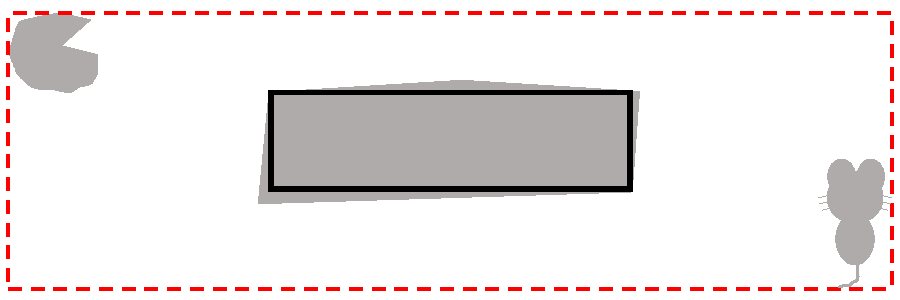
\includegraphics[width=3in]{fig.pdf}
\caption{Example where the underlying distribution $p$ is uniform over the (gray) valid regions. The solid rectangle maximizes our objective since it does not output nonsense (is supported only within the grey matter) and is closest to the $p$ (covers the maximum amount of grey matter). In contrast, the standard maximum likelihood (dashed red) rectangle must fully contain the observed samples, thus generating invalid points most of the time.  }
\end{figure}

Motivated by these observations, we evaluate a generative model $q$ on two axes. First is {\em coverage}, which is related to the probability assigned to future examples drawn from the true distribution $p$. Second is {\em validity}, defined as the probability that random examples generated from $q$ meet some validity requirement. Formally, we measure coverage in terms of a bounded {\em loss}:
$$\Loss(p,q)=\E_{x \sim p}[L(q_x)],$$
where $L:[0,1]\rightarrow [0,M]$ is a bounded decreasing function such as the capped log-loss $L(q_x)=\min(M, \log 1/q_x)$. % or $L(q_x)=\log 1/(q_x+\exp(-M))$. 
A bounded loss has the advantages of being efficiently estimable, and also it enables a model to assign 0 probability to one example (e.g., an outlier or error) if it greatly increases the likelihood of all other data. Validity is defined with respect to a set $V \subseteq X$, and $q(V)$ is the probability that a random example generated from $q$ lies within $V$. 

Clearly, there is a tradeoff between coverage and validity. We first focus on the case of (near) perfect validity. A Valid Generative Modeling (VGM) algorithm if it outputs, for a family of distributions $Q$ over $X$, if it outputs $\hat{q}$ with (nearly) perfect validity and whose loss is nearly as good as the loss of the best valid $q\in Q$. More precisely, $A$ is a VGM learner of $Q$ if for any nonempty valid subset $V \subseteq X$, any probability distribution $p$ over $V$, and any $\eps>0$, $A$ uses $n$ random samples from $p$ and makes $m$ membership oracle calls to $V$ and outputs a distribution $\hat{q}$ such that, $$\Loss(p, \hat{q}) \leq \min_{q \in Q: q(V)=1}\Loss(p,q) + \eps ~\text{ and }~\hat{q}(V)\geq 1-\eps.$$ 
We aim for our learner to be sample and query efficient, requiring that $n$ and $m$ are polynomial in $M, 1/\eps$ and a measure of complexity of our distribution class $Q$.
Furthermore, we would like our algorithms to be computationally efficient, with a runtime polynomial in the size of the data, namely the $n + m$ training examples. 
A more formal description of the problem is available in Section~\ref{sec:problem}.

$A$ is said to be {\em proper} if it always outputs $\hat{q}\in Q$ and {\em improper} otherwise.
In Section~\ref{sec:impossibility}, we first show that efficient proper learning for VGM is impossible. This is an information-theoretic result, meaning that even given infinite runtime and positive samples, one still cannot solve the VGM problem. Interestingly, this is different from binary classification, where it is possible to statistically learn from iid examples without a membership oracle.

Our first main positive result is an efficient (improper) learner for VGM. The algorithm relies on a subroutine that solves the following {\em Generative Modeling with Negatives} (GMN) problem: given sets $X_P, X_N \subset X$ of positive and negative examples, find the probability distribution $q \in Q$ which minimizes $\sum_{x \in X_P} L(q(x))$ subject to the constraint that $q(X_N)=0$. For simplicity, we present our algorithm for the case that the distribution family $Q$ is finite, giving sample and query complexity bounds that are logarithmic in terms of $|Q|$. However, as we show in Section~\ref{sec:infinite-families}, all of our results extend to infinite families $Q$. It follows that if one has a computationally efficient algorithm for the GMN problem for a distribution family $Q$, then our reduction gives a computationally efficient VGM learning algorithm for $Q$.

Our second positive result is an algorithm that minimizes $\Loss(p,q)$ subject to a relaxed validity constraint comparing against the optimal distribution that has validity $q(V)$ at least $1-\alpha$ for some $\alpha>0$. We show in Section~\ref{sec:partial-validity} that even in this more general setting, it is possible to obtain an algorithm that is statistically efficient but may not be computationally efficient. An important open question is whether there exists a computationally efficient algorithm for this problem when given access to an optimization oracle, as was the case for our algorithm for VGM.

\subsection{Related Work}
\cite{KearnsMRRSS94} showed how to learn distributions from positive examples in the realizable setting, i.e., where the true distribution is assumed to belong to the class being learned. In the same sense as their work is similar to PAC learning \citet{Valiant84} of distributions, our work is like agnostic learning \citet{KearnsSS94} in which no assumption on the true distribution is made. 

Generative Adversarial Networks (GANs)~\cite{GoodfellowPMXWOCB14} are an approach for generative modeling from positive examples alone, in which a generative model is trained against a discriminator that aims to distinguish real data from generated data. In some domains, GANs have been shown to outperform other methods at generating realistic-looking examples. Several shortcomings of GANs have been observed \citet{AroraRZ18}, and GANs are still subject to the theoretical limitations we argue are inherent to any model trained without a validity oracle. 

In supervised learning, there is a rich history of learning theory with various types of queries, including membership which are not unlike our (in)validity oracle. Under various assumptions, queries have been shown to facilitate the learning of complex classes such as finite automata \citet{Angluin88} and DNFs \citet{Jackson97}. See the survey of \cite{Angluin92} for further details.  Interestingly, \cite{Feldman09} has shown that for agnostic learning, i.e., without making assumptions on the generating distribution, the addition of membership queries does not enhance what is learnable beyond random examples alone. 
Supervised learning also has a large literature around active learning, showing how the ability to query examples reduces the sample complexity of many algorithms. See the survey of \cite{Hanneke14}. Note that the aim here is typically to save examples and not to expand what is learnable.
 
More sophisticated models, e.g., involving neural networks, can mitigate the invalidity problem as they often generate more realistic natural language and have even been demonstrated to generate \LaTeX{} that nearly compiles \citep{Karpathy15} or nearly valid Wikipedia markdown. However, longer strings generated are unlikely to be valid. For example, \cite{Karpathy15} shows generated markdown which includes:
\begin{quote}
==Access to ''rap===
The current history of the BGA has been [[Vatican Oriolean Diet]], British Armenian, published in 1893.  While actualistic such conditions such as the [[Style Mark Romanians]] are still nearly not the loss.
\end{quote}

Even ignoring the mismatched quotes and equal signs, note that this example has two so-called ``red links'' to two pages that do not exist. Without checking, it was not obvious to us whether or not Wikipedia had pages titled {\em Vatican Oriolean Diet} or {\em Style Mark Romanians}. In some applications, one may or may not want to disallow red links. In the case that they are considered valid, one may seek a full generative model of what might plausibly occur inside of brackets, as the neural network has learned in this case. If they are disallowed, a model might memorize links it has seen but not generate new ones. A validity oracle can help the learner identify what it should avoid generating.

 In practice, \cite{KusnerPH17} discuss how generative models from neural networks (in particular autoencoders) often generate invalid sequences. 
\cite{JanzWPKH18} learn the validity of examples output by a generative model using oracle feedback. 

%!TEX root = main.tex
\vspace{-.0cm}
\section{Preliminaries}\label{sec:background}
\vspace{-1.22pt}
We recall some important concepts from Riemannian geometry. \citet{do2016differential}  provides more a thorough review, with \citet{absil2009optimization} providing a perspective particularly relevant for Riemannian optimization.

As a base space we consider a Riemannian manifold $(\M, \g)$--a smooth manifold equipped with a Riemannian metric $\g$ containing a compact, connected subset $\X$. At all $x \in \M$, the metric $\g$ induces a natural inner product on the tangent space $T_{x} \M$, denoted by $\langle\cdot,\cdot\rangle$--this inner product induces a norm on each tangent space denoted by $\Vert \cdot \Vert$. The metric $\g$ also provides a means of measuring the length of a parametrized curve from $\mathbb{R}$ to the manifold; a \emph{geodesic} is a constant speed curve $\gamma\! :\! [0,1]\! \to\! \M$ that is locally distance-minimizing with respect to the distance~$d$ induced by $\g$.

When considering functions $f : \M \to \mathbb{R}$ we will use $\nabla f(x) \in T_{x} M$ to denote the \emph{Riemannian gradient} of $f$ at $x \in \M$, and $\Hess f(x) : T_{x} M \to T_{x} M$, the \emph{Riemannian Hessian} of $f$ at $x$. When considering functions between manifolds $F : \M \to \M$, we will use $D F(x) : T_{x} \M \to T_{F(x)} \M$ to denote the \emph{differential} of the mapping at $x$ (its linearization) % for which the chain rule and inverse function theorem also hold
\citep[see][for more formal definitions of these objects]{absil2009optimization}.
 \begin{figure}[!t]
 \vspace{-.5cm}
\centering
\begin{minipage}[c]{.48\linewidth}
 \def\svgwidth{2.5in}
%!TEX root = ../colt2018-manifold.tex

%% Creator: Inkscape inkscape 0.92.2, www.inkscape.org
%% PDF/EPS/PS + LaTeX output extension by Johan Engelen, 2010
%% Accompanies image file 'retraction.pdf' (pdf, eps, ps)
%%
%% To include the image in your LaTeX document, write
%%   \input{<filename>.pdf_tex}
%%  instead of
%%   \includegraphics{<filename>.pdf}
%% To scale the image, write
%%   \def\svgwidth{<desired width>}
%%   \input{<filename>.pdf_tex}
%%  instead of
%%   \includegraphics[width=<desired width>]{<filename>.pdf}
%%
%% Images with a different path to the parent latex file can
%% be accessed with the `import' package (which may need to be
%% installed) using
%%   \usepackage{import}
%% in the preamble, and then including the image with
%%   \import{<path to file>}{<filename>.pdf_tex}
%% Alternatively, one can specify
%%   \graphicspath{{<path to file>/}}
%% 
%% For more information, please see info/svg-inkscape on CTAN:
%%   http://tug.ctan.org/tex-archive/info/svg-inkscape
%%
\begingroup%
  \makeatletter%
  \providecommand\color[2][]{%
    \errmessage{(Inkscape) Color is used for the text in Inkscape, but the package 'color.sty' is not loaded}%
    \renewcommand\color[2][]{}%
  }%
  \providecommand\transparent[1]{%
    \errmessage{(Inkscape) Transparency is used (non-zero) for the text in Inkscape, but the package 'transparent.sty' is not loaded}%
    \renewcommand\transparent[1]{}%
  }%
  \providecommand\rotatebox[2]{#2}%
  \ifx\svgwidth\undefined%
    \setlength{\unitlength}{198.42519685bp}%
    \ifx\svgscale\undefined%
      \relax%
    \else%
      \setlength{\unitlength}{\unitlength * \real{\svgscale}}%
    \fi%
  \else%
    \setlength{\unitlength}{\svgwidth}%
  \fi%
  \global\let\svgwidth\undefined%
  \global\let\svgscale\undefined%
  \makeatother%
  \begin{picture}(1,1)%
    \put(0,0){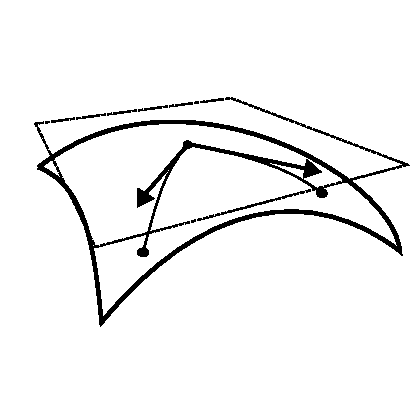
\includegraphics[width=\unitlength,page=1]{Figs/retractionbis.pdf}}%
    \put(0.47046491073,0.658059720226){\color[rgb]{0,0,0}\makebox(0,0)[lb]{\smash{$x_{n-1}$}}}%
     \put(0.75,0.60){\color[rgb]{0,0,0}\makebox(0,0)[lb]{\smash{$-\!\gamma_{n}\nabla f_{n}(x_{n-1})$}}}%
    \put(0.050473214,0.74160431){\color[rgb]{0,0,0}\makebox(0,0)[lb]{\smash{$T_{x_{n-1}}\M$}}}%
    \put(0.88081831845,0.328726181){\color[rgb]{0,0,0}\makebox(0,0)[lb]{\smash{$\M$}}}%
    \put(0.2809223052,0.47167483){\color[rgb]{0,0,0}\makebox(0,0)[lb]{\smash{$v$}}}%
     \put(0.780809223052,0.490167483){\color[rgb]{0,0,0}\makebox(0,0)[lb]{\smash{$x_{n}$}}}%
    \put(0.2207857,0.3651749994){\color[rgb]{0,0,0}\makebox(0,0)[lb]{\smash{$R_{x_{n\!-\!1}}\!(v)$}}}%
  \end{picture}%
\endgroup%

   \end{minipage}
   \begin{minipage}[c]{.48\linewidth}
 \def\svgwidth{2.5in}
%!TEX root = ../colt2018-manifold.tex

%% Creator: Inkscape inkscape 0.92.2, www.inkscape.org
%% PDF/EPS/PS + LaTeX output extension by Johan Engelen, 2010
%% Accompanies image file 'transport.pdf' (pdf, eps, ps)
%%
%% To include the image in your LaTeX document, write
%%   \input{<filename>.pdf_tex}
%%  instead of
%%   \includegraphics{<filename>.pdf}
%% To scale the image, write
%%   \def\svgwidth{<desired width>}
%%   \input{<filename>.pdf_tex}
%%  instead of
%%   \includegraphics[width=<desired width>]{<filename>.pdf}
%%
%% Images with a different path to the parent latex file can
%% be accessed with the `import' package (which may need to be
%% installed) using
%%   \usepackage{import}
%% in the preamble, and then including the image with
%%   \import{<path to file>}{<filename>.pdf_tex}
%% Alternatively, one can specify
%%   \graphicspath{{<path to file>/}}
%% 
%% For more information, please see info/svg-inkscape on CTAN:
%%   http://tug.ctan.org/tex-archive/info/svg-inkscape
%%
\begingroup%
  \makeatletter%
  \providecommand\color[2][]{%
    \errmessage{(Inkscape) Color is used for the text in Inkscape, but the package 'color.sty' is not loaded}%
    \renewcommand\color[2][]{}%
  }%
  \providecommand\transparent[1]{%
    \errmessage{(Inkscape) Transparency is used (non-zero) for the text in Inkscape, but the package 'transparent.sty' is not loaded}%
    \renewcommand\transparent[1]{}%
  }%
  \providecommand\rotatebox[2]{#2}%
  \ifx\svgwidth\undefined%
    \setlength{\unitlength}{198.42519685bp}%
    \ifx\svgscale\undefined%
      \relax%
    \else%
      \setlength{\unitlength}{\unitlength * \real{\svgscale}}%
    \fi%
  \else%
    \setlength{\unitlength}{\svgwidth}%
  \fi%
  \global\let\svgwidth\undefined%
  \global\let\svgscale\undefined%
  \makeatother%
  \begin{picture}(1,1)%
    \put(0,0){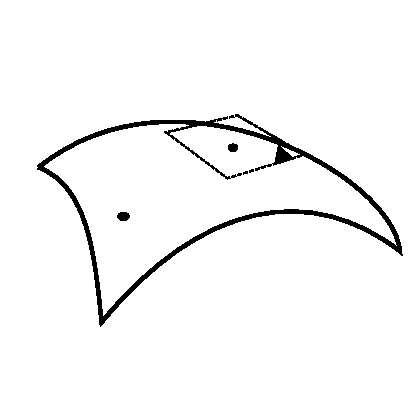
\includegraphics[width=\unitlength,page=1]{Figs/transport2.pdf}}%
    \put(0.88081831845,0.328726181){\color[rgb]{0,0,0}\makebox(0,0)[lb]{\smash{$\M$}}}%
    \put(0,0){\includegraphics[width=\unitlength,page=2]{Figs/transport2.pdf}}%
    \put(0.49373014,0.651988096){\color[rgb]{0,0,0}\makebox(0,0)[lb]{\smash{$x$}}}%
    \put(0.236627,0.47247038){\color[rgb]{0,0,0}\makebox(0,0)[lb]{\smash{$y$}}}%
    \put(0.1720032738,0.6014499){\color[rgb]{0,0,0}\makebox(0,0)[lb]{\smash{$T_y\M$}}}%
    \put(0.594176587,0.7369925609){\color[rgb]{0,0,0}\makebox(0,0)[lb]{\smash{$T_x\M$}}}%
    \put(0.70539679,0.56444469){\color[rgb]{0,0,0}\makebox(0,0)[lb]{\smash{$v$}}}%
    \put(0.42325397,0.4704097231){\color[rgb]{0,0,0}\makebox(0,0)[lb]{\smash{$\tp{x}{y}(v)$}}}%
  \end{picture}%
\endgroup%

  \end{minipage}
  \vspace{-1cm}
\caption{Left: In the tangent space at iterate $x_{n-1}$, a retraction along an arbitrary vector $v$ generating a curve pointing in the ``direction'' of  $v$, and a retraction along the gradient update to $x_n$. Right:
The parallel transport of a different $v$ along the same path.}
\label{fig:manifold}
  \vspace{-.5cm}
\end{figure}
The \emph{exponential map} $\Exp_{x}(v) : T_{x} \M \to \M$ maps $v \in T_{x} \M$ to $y \in \M$ such that there is a geodesic with $\gamma(0)=x$, $\gamma(1)=y$, and $\frac{d}{dt}\gamma(0)=v$; although it may not be defined on the whole tangent space. If there is a unique geodesic connecting $x, y \in \X$, the exponential map will have a well-defined inverse $\Exp_{x}^{-1}(y) : \M \to T_{x}\M$, such that the length of the connecting geodesic is $d(x,y)=\Vert \Exp_{x}^{-1}(y) \Vert$. We also use $R_x : T_{x} \M \to \M$ and $R_x^{-1} : \M \to T_{x}\M$ to denote a \emph{retraction mapping} and its inverse (when well defined), which is an approximation to the exponential map (and its inverse). $R_x$ is often computationally cheaper to compute then the entire exponential map $\Exp_x$. Formally, the map $R_x$ is defined as a first-order retraction if $R_x(0) = x$ and $D R_x(0)= id_{T_{x} \M}$---so locally $R_x(\xi)$ must move in the ``direction'' of $\xi$. The map $R_x$ is a second-order retraction if $R_x$ also satisfies $\frac{D^2}{dt^2} R_x(t \xi)|_{0} = 0$ for all $\xi \in T_{x}\M$, where $\frac{D^2}{dt^2}\gamma = \frac{D}{dt} \dot{\gamma}$ denotes the acceleration vector field \citep[][Sec.~5.4]{absil2009optimization}. This condition ensures $R_x$ satisfies a ``zero-acceleration'' initial condition.
Note that locally, for $x$ close to $y$, the retraction satisfies $\norm{R^{-1}_{x}(y)} = d(x, y) + o(d(x, y))$.

If we consider the example where the manifold is a sphere (i.e., $\M = S^{d-1}$ with the round metric $\g$), the exponential map along a vector will generate a curve that is a great circle on the underlying sphere. A nontrivial example of a retraction $R$ on the sphere can be defined by first moving along the tangent vector in the embedded Euclidean space $\mathbb{R}^d$, and then projecting this point to the closest point on the sphere.

We further define the \emph{parallel translation} $\tp{x}{y} : T_x \mathcal{M} \to T_y \mathcal{M}$ as the map
transporting a vector $v \in T_x \M$ to $\tp{x}{y} v$, along a path $R_{x}(\xi)$ connecting $x$ to $y = R_{x}(\xi)$, such that the vector stays ``constant" by satisfying a zero-acceleration condition. This is illustrated in \myfig{manifold}. The map $\tp{x}{y}$ is an isometry. We also consider, a different vector transport map $\te{x}{y}:T_x \mathcal{M} \to T_y \mathcal{M}$ which is the differential  $DR_{x}(R_x^{-1}(y))$ of the retraction $R$ \citep[][Sec.~8.1]{absil2009optimization}.

Following \citet{huang2015broyden}, we will call a function $f$ on $\X$ \emph{retraction convex} on $\X$ (with respect to $R$) if for all $x \in \X$ and all $\eta \in T_{x}\M$ satisfying $\norm{\eta}=1$, $t \mapsto f(R_{x}(t \eta))$ is convex for all $t$ such that $R_{x}(t \eta) \in \X$; similarly $f$ is \emph{retraction strongly convex} on $\X$ if $t \mapsto f(R_{x}(t \eta))$ is strongly convex under the same conditions. If $R_x$ is the exponential map, this reduces to the definition of geodesic convexity \citep[see the work of][for further details]{zhang2016first}.
\vspace{-1.21pt}
\section{Assumptions} \label{sec:assumptions}
\vspace{-1.22pt}
We introduce several assumptions on the manifold $\M$, function $f$, and the noise process $\{\nabla f_n\}_{n\geq1}$ that will be relevant throughout the paper.
\vspace*{-.1850cm}
\subsection{Assumptions on $\M$}
\vspace{-.0856cm}
First, we assume the iterates of the algorithm in \eq{grad_desc} and \eq{ave_grad_desc}
remain in $\mathcal X$ where the manifold ``behaves well.'' Formally,
\vspace*{-4pt}
\begin{assumption} \label{assump:manifold}
  For a sequence of iterates $\{ x_n \}_{n \geq 0}$ defined in \eq{grad_desc}, there exists a compact, connected subset $\mathcal X$ such that $x_n \in \mathcal X$ for all $n \geq 0$, and $x_\star \in \mathcal X$. Furthermore, $\mathcal X$ is totally retractive (with respect  to the retraction $R$) and the function $x\mapsto \Vert \frac{1}{2} R_y^{-1}(x)\Vert^2$ is retraction strongly convex on $\X$ for all $y\in\X$. Also, $R$ is a second-order retraction at $x_\star$.
\end{assumption}
\vspace*{-4pt}
Assumption~\ref{assump:manifold} is restrictive, but standard in prior work on stochastic approximation on manifolds \cite[e.g.,][]{bonnabel2013stochastic, zhang2016riemannian, sato2017riemannian}.
As further detailed by \citet{huang2015broyden}, a totally retractive neighborhood $\X$ is such that
for all $x \in \X$ there exists $r>0$ such that $\X \subset R_{x} (\mathbb{B}_{r}(0))$
where $R_x$ is a diffeomorphism on $\mathbb{B}_{r}(0)$. A totally retractive neighborhood is analogous to the concept of a totally normal neighborhood \citep[see, e.g.,][Chap. 3, Sec. 3]{do2016differential}.
Principally, Assumption~\ref{assump:manifold} ensures that the retraction map (and its respective inverse) are well-defined when applied to the iterates of our
algorithm.

If $\M$ is a Hadamard manifold, the exponential map (and its inverse) is defined everywhere on~$\M$, although this globally may not
be true for a retraction $R$. Similarly, if $\M$ is a compact manifold the first statement of Assumption~\ref{assump:manifold} is always satisfied. Moreover, in the case of the exponential map, $x \mapsto \frac{1}{2} \Vert \Exp_y^{-1}(x)\Vert^2$ is strongly convex in a ball around $y$
whose radius depends on the curvature, as explained by \citet{Afs11} and \citet[Ch. IV, Sec. 2 Lemma 2.9]{Sak96}. For our present purpose, we also assume the retraction $R$ agrees with the Riemannian exponential map up to second order near $x_\star$. This assumption, that $R$ is a second-order retraction, is fairly general and is satisfied by projection-like retraction maps on matrix manifolds \citep[see][]{AbsMal12}.
\vspace*{-.8cm}
\subsection{Assumptions on $f$}
\vspace{-.0856cm}
We now introduce some regularity assumptions on the function $f$ ensuring
sufficient differentiability and strong convexity at $x_\star$:
\begin{assumption} \label{assump:strongconvpoint}
The function $f$ is twice-continuously differentiable on $\X$. Further
the Hessian of the function $f$ at $x_\star$, $\Hess f(x_\star)$, satisfies,
for all $v \in T_{x_\star}\M$ and $\mu>0$,
\[
\langle v, \Hess f(x_\star)v\rangle \geq \mu \Vert v\Vert^2>0.
\]
\end{assumption}
Continuity of the Hessian  also ensures local retraction strong convexity in a neighborhood of $x_\star$ \citep[][Prop. 5.5.6]{absil2009optimization}. Moreover, since the function $f$ is twice-continuously differentiable on $\X$ its Hessian is Lipschitz on this compact set.
We formalize this as follows:
\begin{assumption}  \label{assump:HessianLip}
 There exists $M>0$ such that the Hessian of the function $f$, $\Hess f$, is $M$-Lipschitz  at $x_\star$.
That is, for all $y \in \X$ and $v \in T_{y}\M$,
\[
\Vert \tp{y}{x_\star}  \circ \Hess f(y) \circ \tp{x_\star}{y} -  \Hess f(x_\star)\Vert_{op} \leq M \Vert R_{x_\star}^{-1}(y) \Vert.
\]
\end{assumption}
Note that $\Vert R_{x_\star}^{-1}(y) \Vert$ is not necessarily symmetric under the exchange of $x_\star$ and $y$. This term could also be replaced with $d(x_\star, y)$, since these expressions will be locally equivalent
in a neighborhood of $x_\star$, but would come at the cost of a less transparent analysis.
\vspace{-0.11pt}
\subsection{Assumptions on the noise} \label{sec:assumptions_noise}
\vspace{-.0856cm}
We state several assumptions on the noise process that will be relevant throughout our discussion.
Let $(\F_n)_{n \geq 0}$ be an increasing sequence of sigma-fields. We will assume access to a sequence $\{\nabla f_n\}_{n \geq 1}$
of noisy estimates of the true gradient $\nabla f$ of the function $f$,
\begin{assumption} \label{assump:noiseunbiased}
The sequence of (random) vector fields $\{ \nabla f_n \}_{n\geq1} : \mathcal M \to T\mathcal M$ is $\F_n$-measurable, square-integrable and unbiased:
    \[
\forall x \in \X, \ \forall n \geq 1, \ \E[\nabla f_n(x)\vert \F_{n-1}]=\nabla f(x).
\]
\end{assumption}
This general framework subsumes two situations of interest.
\begin{itemize}
 \vspace*{-6pt}
 \item
Statistical Learning (on Manifolds): minimizing a loss function $\ell: \mathcal M \times  \mathcal Z \to \mathbb R$ over $x \in \mathcal X$, given a sequence
of i.i.d. observations in $\mathcal Z$, with access only to noisy, unbiased estimates of the gradient $\nabla f_n=\nabla \ell(\cdot,z_n)$ \citep{AswBicTom11}.
\vspace*{-6pt}
\item
Stochastic Approximation (on Manifolds): minimizing a function $f(x)$ over $x \in \mathcal X$, with access only to the
(random) vector field $\nabla f(x) + \epsilon_n(x)$ at each iteration. Here the gradient vector field is perturbed
 by a square-integrable martingale-difference sequence (for all $x\in\mathcal M $, $\E[\epsilon_n(x) \vert \F_{n-1}]=0$) \citep{bonnabel2013stochastic}.
\end{itemize}
Lastly, we will assume the vector fields $\{\nabla f_n\}_{n \geq 1}$ are individually Lipschitz and have
bounded covariance at the optimum $x_\star$:
\vspace*{-4pt}
\begin{assumption} \label{assump:noiseLip}
 There exists $L > 0$ such that for all $x \in \mathcal X$ and $n\geq 1$, the vector field $\nabla f_n$ satisfies
\[ \E [\Vert  \tp{x}{x_\star} \nabla f_n(x)- \nabla f_n(x_\star)\Vert^2\vert  \F_{n-1}]\leq L^2 \ \Vert R_{x_\star}^{-1}(x) \Vert^2 ,
 \]
there exists $\tau>0$ such that $ \E [\Vert  \nabla f_{n}(x) \Vert^4\vert  \F_{n-1}]\leq \tau^4$ for all $x \in \X$, and a symmetric positive-definite matrix $\Sigma$ such that,
 \[
 \E[\nabla f_n(x_\star) \otimes \nabla f_n(x_\star) \vert\mathcal F_{n-1}] = \Sigma \text{ a.s.} \]
\end{assumption}
These are natural generalizations of standard assumptions in the optimization literature \citep{Fab68} to the setting of
Riemannian manifolds\footnote{Assuming bounded gradients does not contradict Assumption~\ref{assump:strongconvpoint}, since we are constrained to the compact set $\X$.}. Note that the assumption, \\ $\E[\nabla f_n(x_\star) \otimes \nabla f_n(x_\star) \vert\mathcal F_{n-1}] = \Sigma \text{ a.s.}$ could be slightly relaxed (as detailed in \myapp{conv_rates}),
but allows us to state our main result more cleanly.

%!TEX root = colt2018.tex

We now consider results on (averaged) SGD for least-squares that are interesting on their own. As said before, we show  results in two different settings depending on the step-size sequence. First,  we consider $(\gamma_n)$ as a decreasing sequence, second we take $(\gamma_n)$ constant but prove the convergence of the (tail-)averaged iterates.

Since the results we need could be of interest (even for finite-dimensional models), in this section, we study the following general recursion:
\begin{align}
\label{eq:SGDabstract}
\eta_n = ( \idm - \gamma H_n) \eta_{n-1} + \gamma_n \varepsilon_n,
\end{align}
%
We make the following assumptions:  
\vspace{-0.2cm}
%
\basgd \label{asm:init}  We start at some $\eta_0 \in \H$. \easgd
\vspace{-0.65cm}
\basgd \label{asm:noise-iid}   $(H_n,\varepsilon_n)_{n \geqslant 1} $ are  i.i.d. and $H_n$ is a positive self-adjoint operator so that almost surely $H_n \succcurlyeq \lambda \idm$, and $H  := \E H_n$. \easgd
\vspace{-0.5cm}
\basgd \label{asm:noise-bound}  Noise: $ \E  \varepsilon_n   = 0$, $\| \varepsilon_n  \|_\H \leqslant c^{1/2} $ almost surely and $\E  ( \varepsilon_n   \otimes \varepsilon_n ) \preccurlyeq C$, with $C$ commuting with $H$. Note that one consequence of this assumption is $\E \|\varepsilon_n\|_\H^2 \leqslant \tr C$. \easgd
\vspace{-0.5cm}
\basgd \label{asm:weird-bound}  For all $n \geqslant 1$, $\E \Big[  H_n C H^{-1} H_n \Big] \preccurlyeq \gamma_0^{-1} C$ and $\gamma \leqslant \gamma_0$. \easgd
\vspace{-0.5cm}
\basgd \label{asm:commute}  $A$ is a positive self-adjoint operator which commutes with $H$. \easgd
%
Note that we will later apply the results of this section to $H_n =  K_{x_n} \otimes K_{x_n} + \lambda I$, $H = \Sigma + \lambda \idm$, $C = \Sigma$ and $A \in \{\idm, \Sigma\}$. We first consider the non-averaged SGD recursion, then the (tail-)averaged recursion. The key difference with existing bounds is the need for precise probabilistic deviation results.


For least-squares, one can always separate the impact of the initial condition $\eta_0$ and of the noise terms $\varepsilon_k$, namely $\eta_n = \eta_n^{\textrm {bias}} + \eta_n^{\textrm {variance}}$, where $\eta_n^{\textrm {bias}}$ is the recursion with no noise ($\varepsilon_k = 0$), and $\eta_{n}^{\textrm {variance}}$ is the recursion started at $\eta_0=0$. The final performance will be bounded by the sum of the two separate performances \citep[see, e.g.,][]{defossez2014constant}. Hence all of our bounds will depend on these two. See more details in Appendix \ref{sec:AppSGD}.


\subsection{Non-averaged SGD}

In this section, we prove results for the recursion defined by Eq.~\eqref{eq:SGDabstract} in the case where for $\alpha \in [0,1]$, $ \gamma_n = \gamma/n^\alpha$. These results extend the ones of \citet{gradsto} by providing deviation inequalities, but are limited to least-squares. For general loss functions and in the strongly-convex case, see also~\citet{kakade2009generalization}.

\begin{theorem}[SGD, decreasing step size: $\gamma_n = \gamma/n^\alpha$] \label{th:SGDalpha}
Assume \sgdasm{asm:init}, \sgdasm{asm:noise-iid}, \sgdasm{asm:noise-bound}, $\gamma_n = \gamma/n^\alpha$, $\gamma\lambda < 1$ and denote by $\eta_n \in \H$ the n-th iterate of the recursion in Eq. \eqref{eq:SGDabstract}. We have for $t > 0, n \geqslant 1$ and  $\alpha \in (0,1)$, $\|g_n - g_\lambda\|_\H \leqslant \exp\left(  -\frac{\gamma\lambda}{1-\alpha}\left( (n+1)^{1-\alpha} -1  \right)   \right) \|g_0 - g_\lambda\|_\H + V_n$, almost surely for~$n$ large enough \footnote {See Appendix Section \ref{sec:AppSGD} Lemma \ref{le:nalpha} for more details.}, with
$\displaystyle \P \left( V_n \geqslant t \right) \leqslant 2\exp\left( -\frac{ t^2 }{ 8 \gamma \tr C/\lambda  + \gamma c^{1/2}t }\cdot n^{\alpha}\right).$
\end{theorem}
%
We can make the following observations: 
\vspace{-0.1cm}
\BIT
\itemsep-3pt
\item The proof technique (see Appendix \ref{ap:SGDalpha} for the detailed proof) relies on the following scheme: we notice that $\eta_n$ can be decomposed in two terms, (a) the bias: obtained from a product of $n$ contractant operators, and (b) the variance: a sum of increments of a martingale. We treat separately the two terms. For the second one, we prove almost sure bounds on the increments and on the variance that lead to a Bernstein-type concentration result on the tail $\P (V_n \geqslant t)$. Following this proof technique, the coefficient in the latter exponential is composed of the variance bound plus the almost sure bound of the increments of martingale times $t$.
%
\item Note that we only presented in Theorem \ref{th:SGDalpha} the case where $\alpha \in (0,1)$. Indeed, we only focused on the case where we had exponential convergence (see the whole result in the Appendix: Proposition \ref{prop:fullalpha}). Actually, that there are three different regimes. For $\alpha=0$ (constant step-size), the algorithm is not converging, as the tail probability bound on $\P \left( V_n \geqslant t \right) $ is not dependent on $n$. For $\alpha=1$, confirming results from~\citet{gradsto}, there is no exponential forgetting of initial conditions. And for $\alpha \in (0,1)$, the forgetting of initial conditions and the tail probability are converging to zero exponentially fast, respectively,  as $\exp( - C n^{1-\alpha})$ and $\exp( - C n^{\alpha})$, for a constant $C$, hence the natural choice of $\alpha=1/2$ in our experiments.

\EIT

\subsection{Averaged and Tail-averaged SGD with constant step-size}
 
In the subsection, we take: $\forall n \geqslant 1, \ \gamma_n = \gamma$. We first start with a result on the variance term, whose proof extends the work of \citet{daft} to deviation inequalities which are sharper than the ones from \cite{newsto}.


\begin{theorem}[Convergence of the variance term in averaged SGD]
\label{th:SGDaveraged}
Assume \sgdasm{asm:init}, \sgdasm{asm:noise-iid}, \sgdasm{asm:noise-bound},$\ $ \sgdasm{asm:weird-bound}, \sgdasm{asm:commute} and consider the average of the $n+1$ first iterates of the sequence defined in Eq. \eqref{eq:SGDabstract}: $\bar{\eta}_n = \frac{1}{n+1} \sum_{i=0}^n \eta_i$. Assume $\eta_0 = 0$.
 We have for $t > 0, n \geqslant 1$:    
\begin{equation}
\displaystyle\P \left( \left\| A^{1/2} \bar{\eta}_n  \right\|_\H \geqslant t \right) \leqslant 2 \exp\left[-\frac{(n+1) t^2}{E_t}\right],
\end{equation}
where $E_t$ is defined with respect to the constants introduced in the assumptions:  
\begin{equation}
\label{eq:Et}
 E_t =   4\tr(AH^{-2}C)+\frac{2c^{1/2} \|A^{1/2}\|_{\textrm {op}}}{3\lambda}\cdot t  .
 \end{equation}
\end{theorem}
%
The work that remains to be done is to bound the bias term of the recursion $\bar{\eta}_n^{\textrm {bias}}$. We have done it for the full averaged sequence (see Appendix \ref{ap:SGDfullaverage} Theorem \ref{th:withbias}) but as it is quite technical and could lower a bit the clarity of the reasoning, we have decided to leave it in the Appendix. We present here another approach and consider the tail-averaged recursion, $\bar{\eta}_n^{\textrm {tail}} 
= \frac{1}{\lfloor n/2 \rfloor} \sum_{i=\lfloor n/2 \rfloor}^{n} \eta_i$ \citep[as proposed by][]{jain2016parallelizing,shamir2011SGD}.
%
For this, we use the simple almost sure bound
$ \| \eta_i^{\textrm {bias}} \|_\H \leqslant ( 1- \lambda \gamma )^i \|\eta_0\|_\H$, such that 
$\| \bar{\eta}_n^{\textrm {tail, bias}} \|_\H \leqslant ( 1- \lambda \gamma )^{n/2} \|\eta_0\|_\H$. For the variance term, we can simply use the result above for $n$ and $n/2$, as 
$\bar{\eta}_n^{\textrm {tail}}  = 2 \bar{\eta}_n  - \bar{\eta}_{n/2}$. This leads to:
 \clearpage
 \begin{corollary}[Convergence of tail-averaged SGD]
 \label{co:SGDtailaveraged}
Assume \sgdasm{asm:init}, \sgdasm{asm:noise-iid}, \sgdasm{asm:noise-bound}, \sgdasm{asm:weird-bound}, \sgdasm{asm:commute} and consider the tail-average of the sequence defined in Eq. \eqref{eq:SGDabstract}: $\bar{\eta}_n^{\textrm {tail}} = \frac{1}{\lfloor n/2 \rfloor} \sum_{i=\lfloor n/2 \rfloor}^{n} \eta_i$.
 We have for $t > 0, n \geqslant 1$:   
\begin{eqnarray}
\left\|A^{1/2}\bar{\eta}_n^{\textrm {tail}} \right\|_\H &\leqslant& (1-\gamma\lambda)^{n/2} \|A^{1/2}\|_{op} \|\eta_0\|_\H + L_n \quad,\ \text{with} \\
 \P(L_n \geqslant t ) &\leqslant& 4\exp\left( -  (n+1)t^2 /( 4 E_t)\right),
\end{eqnarray}
where $L_n$ is defined in the proof (see Appendix \ref{ap:SGDcorrolary}) and is the variance term of the tail-averaged recursion.
\end{corollary}
%
We can make the following observations on the two previous results:
\vspace{-0.1cm}
\BIT
\itemsep-3pt
\item The proof technique (see Appendix \ref{ap:SGDaverage} and \ref{ap:SGDcorrolary} for the detailed proofs) relies on concentration inequality of Bernstein type. Indeed, we notice that (in the setting of  Theorem \ref{th:SGDaveraged}) $\bar{\eta}_n$ is a sum of increments of a martingale. We prove almost sure bounds on the increments and on the variance \citep[following the proof technique of][]{daft} that lead to a Bernstein type concentration result on the tail $\P (V_n \geqslant t)$. Following the proof technique summed-up before, we see that $E_t$ is composed of the variance bound plus the almost sure bound times $t$. 
%
\item Remark that classically, $A$ and $C$ are proportional to $H$ for excess risk predictions. In the finite $d$-dimensional setting this leads us to the usual variance bound proportional to the dimension~$d$: $\tr (AH^{-2}C) \cong \tr \idm = d$. The result is general in the sense that we can apply it for all  matrices $A$ commuting with $H$ (this can be used to prove results in $L_2$ or in~$\H$). 
%
\item Finally, note that we improved the variance bound with respect to the strong convexity parameter $\lambda$ which is usually of the order $1/\lambda^2$ \citep[see][]{shamir2011SGD}, and is here $\tr (AH^{-2}C)$. Indeed, in our setting, we will apply it for $A = C = \Sigma$ and $H = \Sigma + \lambda I$, so that $\tr (AH^{-2}C)$ is upper bounded by the effective dimension $\tr (\Sigma (\Sigma + \lambda I)^{-1})$ which can be way smaller than $1/\lambda^2$ \citep[see][]{caponnetto2007optimal,dieuleveut2016nonparametric}.
%
\item The complete proof for the full average is written in Appendix \ref{ap:SGDfullaverage} and more precisely in Theorem \ref{th:withbias}. In this case the initial conditions are not forgotten exponentially fast though.
\EIT




\section{Row-Sparsity Bounds for $\ell_1$ Regression}\label{sec:sparsitypreserve}
In this section, we explain how to avoid using matrix multiplication, which we use in Lemma~\ref{lem:lewisAndRotate}, to get an IRB matrix, and in Lemma~\ref{lem:easyInit}, to get a good initialization. To avoid both procedures, we assume that our given matrix $\AA \in \R^{n\times d}$ and vector $\bb \in \R^{n }$ are such that $[\AA\;\bb]^T [\AA\;\bb] \approx_{O(1)} \II$ and for each row $i$ of $[\AA\;\bb]$ we have $\norme{[\AA\;\bb]_{i,:}}^2 \approx_{O(1)} d/n$. Notice that these conditions imply $\AA^T\AA \approx_{O(1)} \II$ and $\norme{\AA_{i,:}}^2 \leq O(d/n)$, which are nearly the properties of the preconditioned matrix $\tilde{\AA}\UU$ generated in Lemma~\ref{lem:lewisAndRotate}. However, we still face two new complications: (1) the row count of matrix $\AA$ has not been reduced from $n$ to $O(d\epsilon^{-2}\log{n})$, and (2) $\AA$ is only approximately isotropic.

We will account for the first complication by showing that, under these conditions, the Lewis weights are approximately equal, which implies that uniform row sampling is nearly equivalent to that in \Cref{thm:lewisWeights}. 
We then describe how to find a good initialization point using conjugate gradient methods when $\tilde{\AA}$ is only approximately isotropic. 
Finally, we use the reduction in \cite{AllenZhuH16} and the Katyusha stochastic gradient descent algorithm from \cite{AllenZhu17} to achieve a total running time of $\Otil(nnz(\AA) + sd^{1.5}\epsilon^{-2} + d^2\epsilon^{-2})$, where $s$ is the maximum number of non-zeros in a row of $\AA$. Note that as a byproduct of this algorithm, we achieve row-sparsity-preserving $\ell_1$ minimization.


\subsubsection*{Uniform Sampling of $\AA$}
We deal with the first complication of avoiding Lemma~\ref{lem:lewisAndRotate} by sampling $\AA$ uniformly. In particular, if we uniformly sample $N = O(d\epsilon^{-2} \log d)$ rows of $[\AA\;\bb]$, this yields a smaller matrix $[\tilde{\AA}\;\tilde{\bb}]$ such that $\tilde{\AA}^T\tilde{\AA} \approx_{O(1)} \II$ and $\|\tilde{\AA}_{i,:}\|_2^2 \leq  O(d/N)$ for each row $i$, which is to say $\tilde{\AA}$ is almost IRB. This then culminates in the following lemma whose proof we relegate to \Cref{subsec:unifSample}.

\begin{restatable}[]{lemma}{uniformSampling}
	\label{lem:uniformSampling}
	Suppose we are given a matrix $\AA \in \R^{n \times d}$ such that $\AA^T\AA \approx_{O(1)} \II$ and $\norme{\AA_{i,:}}^2 \approx_{O(1)} d/n$.
	If we uniformly sample $N = O(d\epsilon^{-2}\log{n})$ rows independently and rescale each row by $n/N$ to obtain matrix $\tilde{\AA}$, then with high probability the following properties hold:
	\begin{enumerate}
		\item $\norm{\AA\xx}_1 \approx_{1 + \epsilon} \|\tilde{\AA}\xx\|_1$ for all $\xx \in \R^d$.
		\item $\tilde{\AA}^T\tilde{\AA} \approx_{O(1)} \left(\dfrac{n}{N}\right)\II$.
		\item $\|\tilde{\AA}_{i,:}\|_2^2 \approx_{O(1)} dn/N^2$ for all rows $i \in \{1,2,\ldots, N\}$.
	\end{enumerate}
\end{restatable}




%\todo{make this flow after removing some sections}


\subsubsection*{Initialization using Approximate $\ell_2$ Minimizer}\label{subsec:l2Minimizer}
It now remains to show that we can still find a good initialization $\xx_0$ for gradient descent even with our relaxed assumptions on $\AA$.
Previously, when we had $\AA^T \AA = \II$, we used $\xx_0 = \AA^T \bb = \arg \min_{\xx} \norme{\AA \xx - \bb}$.
It turns out that for $\AA^T \AA \approx_{O(1)} \II$, the $\ell_2$ minimizer $\xx_0 = \arg \min_{\xx} \norme{\AA \xx - \bb}$ is still a good initialization point.
But finding an exact $\ell_2$ minimizer would take a prohibitive amount of time or would require matrix multiplication.
However, an approximate $\ell_2$ minimizer suffices, and we can find such a point quickly using the conjugate gradient method.

For this section, we define $\xx^* \defeq \arg\min_{\xx} \norm{\AA\xx - \bb}_1$ and $\xx_0 \defeq \arg \min_{\xx} \norme{\AA\xx - \bb}$. Our main result is the following:

\begin{lemma}[Approximate $\ell_2$ minimizer is close to $x^*$] \label{lem:initMain} Let $\AA \in \R^{n \times d}$ be such that $\AA^T \AA \approx_{O(1)} \II$ and for each row $i$ of $\AA$, $\norme{\AA_{i,:}}^2 \leq O(d/n)$. Assume that $\norme{\bb} \le n^c$ and $\norme{\AA\xx_0 - \bb} \ge n^{-c}$ for some constant $c > 0$.
	\begin{align*}
	\norme{\tilde{\xx}_0 - \xx^*} \le O(\sqrt{d/n}) \norm{\AA \xx^* - \bb}_1.
	\end{align*}
	Moreover, $\tilde{\xx}_0$ can be computed in  $O( (t_{\AA^T \AA} + d) \log (n/ \epsilon))$ time, where $t_{\AA^T \AA}$ denotes the time to multiply a vector by $\AA^T \AA$. 
\end{lemma}

We prove Lemma~\ref{lem:initMain} using the following two lemmas whose proofs are deferred until \Cref{subsec:initialization_proofs}. Lemma~\ref{lem:exactInit} shows that the $\ell_2$ minimizer is close to the $\ell_1$ minimizer even when $\AA$ is only approximately isotropic, and the proof is similar to that of Lemma~\ref{lem:easyInit}.
Lemma~\ref{lem:cg} shows that we can find a good estimate for the $\ell_2$ minimizer.

\begin{lemma}[Exact $\ell_2$ minimizer is close to $\xx^*$]\label{lem:exactInit}
	Let $\AA \in \R^{n \times d}$ be such that $\AA^T \AA \approx_{O(1)} \II$ and for each row $i$ of $\AA$, $\norme{\AA_{i,:}}^2 \leq O(d/n)$. Then
	\begin{align*}
	\norme{\xx_0 - \xx^*} \le O(\sqrt{d/n}) \norm{\AA \xx^* - \bb}_1.
	\end{align*}
\end{lemma}

\begin{lemma}[Conjugate gradient finds an approximate $\ell_2$ minimizer]\label{lem:cg}
Let $\AA \in \R^{n \times d}$ be such that $\AA^T \AA \approx_{O(1)} \II$ and for each row $i$ of $\AA$, $\norme{\AA_{i,:}}^2 \leq O(d/n)$. Assume that $\norme{\bb} \le n^c$ and $\norme{\AA\xx_0 - \bb} \ge n^{-c}$.
Then for any $\epsilon > 0$, the conjugate gradient method can find an $\tilde{\xx}_0$ such that
\begin{align*}
\norme{\tilde{\xx}_0 - \xx_0} \le \epsilon \norme{\AA\xx_0 - \bb}.
\end{align*}
Moreover, $\tilde{\xx}_0$ can be found in time $O( (t_{\AA^T \AA} + d) \log (n/ \epsilon))$, where $t_{\AA^T \AA}$ is the time to multiply a vector by $\AA^T \AA$. 
\end{lemma}

\begin{proof}[Proof of Lemma~\ref{lem:initMain}]
	We use conjugate gradient with $\epsilon = \sqrt{d/n}$ to find an $\tilde{\xx}_0$ in $O((t_{\AA^T \AA} + d) \log (n/ \epsilon))$ time by Lemma~\ref{lem:cg} to achieve our desired initialization time bounds.
	Note that by definition of $\xx_0$ and by a standard norm inequality, we have:
	\begin{align*}
	\norme{\AA \xx_0 - \bb} \le \norme{\AA \xx^* - \bb} \le \norm{\AA \xx^* - \bb}_1
	\end{align*}
	
	Then by the triangle inequality and Lemma~\ref{lem:exactInit} we have:
	\begin{align*}
	\norme{\tilde{\xx}_0 - \xx^*} &\le \norme{\tilde{\xx}_0 - \xx_0} + \norme{\xx_0 - \xx^*} \\
	&\le \sqrt{d/n}\norm{\AA \xx^* - \bb}_1 + O(\sqrt{d/n})\norm{\AA \xx^* - \bb}_1
%\qedhere
	\end{align*}
	which gives our desired initialization accuracy.
\end{proof}

\subsubsection*{Fast Row-sparsity-preserving $\ell_1$ Minimization}

Finally, we combine the matrix achieved by uniform sampling in Lemma~\ref{lem:uniformSampling} and the initialization from Lemma~\ref{lem:initMain} to achieve fast row-sparsity-preserving $\ell_1$ minimization. This then gives the following main theorem that we prove in \Cref{subsec:achievingSparsity}.

\noFastMatrixMult*



%\input{p_norms}
%\input{grad_descent}
%\input{accelerated}	
%\input{technical}

% Acknowledgments---Will not appear in anonymized version
\acks{We are grateful to Richard Peng for many insightful discussions. We would also like to thank Michael Cohen for his helpful comments
	and Junxing Wang for his feedback. We thank the anonymous reviews of an earlier version of this
	manuscript for their very valuable comments, especially with
	regards to the performances of the many existing
	algorithms in the $\ell_1$ case.}


\bibliography{gd}


\appendix
\section{Proof of Theorem~\ref{thm:applyKatyusha}}\label{sec:katyushaproof}

In this section, we prove our primary result, stated in \Cref{thm:applyKatyusha}.
Specifically, we further examine whether our strong initialization distance bound will allow us to improve the running time with black-box accelerated stochastic gradient descent methods.
The first step towards this is to apply smoothing reductions to our objective function.

\subsection{Smoothing the Objective Function and Adding Strong Convexity}

As before, we let $\xx^* = \arg\min_{\xx} \norme{\AA\xx - \bb}$. For clarity, we will borrow some of the notation from \cite{AllenZhuH16} to more clearly convey their black-box reductions.% to reduce the objective function to one with smoothness and strong convexity, along with its corresponding runtime and approximation guarantees.

\begin{definition}
	A function $f(x)$ is $(L,\sigma)$-\textit{smooth-sc} if it is both $L$-\textit{smooth} and $\sigma$-\textit{strongly-convex}.
\end{definition}

\begin{definition}
	An algorithm $\calA(f(x),x_0)$ is a $\textsc{Time}_\calA(L,\sigma)$-\textit{minimizer} if $f(x)$ is  $(L,\sigma)$-\textit{smooth-sc} and $\textsc{Time}_\calA(L,\sigma)$ is the time it takes $\calA$ to produce $x'$ such that $f(x') - f(x^*) \leq \frac{f(x_0) - f(x^*)}{4}$ for any starting $x_0$.
\end{definition}

Allen-Zhu and Hazan assume access to efficient $\textsc{Time}_\calA(L,\sigma)$-\textit{minimizer} algorithms, and show how a certain class of objective functions can be slightly altered to meet the smoothness and strong convexity conditions to apply these algorithms without losing too much in terms of error and runtime.


\begin{theorem}[Theorem C.2 from \cite{AllenZhuH16}]\label{thm:reductionAlgo}
	Consider the problem of minimizing an objective function
	\[f(x) = \frac{1}{n}\sum_{i=1}^n f_i(x) \]
	such that each $f_i(\cdot)$ is $G$-Lipschitz continuous. Let $\xx_0$ be a starting vector such that $f(\xx_0) - f(\xx^*) \leq \Delta$ and $\|\xx_0 - \xx^*\|_2^2 \leq \Theta$. 
	Then there is a routine that takes as input a $\textsc{Time}_\calA(L,\sigma)$-\textit{minimizer}, $\calA$, alongside $f(x)$ and $x_0$, with $\beta_0 = \Delta/G^2$, $\sigma_0 = \Delta/\Theta$ and $T = \log_2(\Delta/\epsilon)$, and produces $x_T$ satisfying $f(x_T) - f(x^*) \leq O(\epsilon)$ in total running time \[\sum_{t=0}^{T-1}\textsc{Time}_{\calA}(2^t/\beta_0,\sigma_0\cdot 2^{-t}).\] 
\end{theorem}


It is then straightforward to show that our objective function fits the necessary conditions to utilize \Cref{thm:reductionAlgo}.


\begin{lemma}\label{lem:minEqualSumLipsFunctions}
	If $\AA$ is IRB, then the function $\norm{\AA\xx - \bb}_1$ can be written as $\frac{1}{n}\sum_{i=1}^n f_i(\xx)$ such that each $f_i(\cdot)$ is $O(\sqrt{nd})$-Lipschitz continuous.
\end{lemma}


\begin{proof}
	By the definition of 1-norm,
	\[\norm{\AA\xx - \bb}_1 = \sum_{i=1}^n\abs{\AA_{i,:}\xx-\bb_i}.\]
	We then set $f_i(\xx) = n \cdot \abs{\AA_{i,:}\xx-\bb_i}$ and the result follows from Lemma~\ref{lem:easyLipscitz}.
\end{proof}

We can then incorporate our objective into the routine from \Cref{thm:reductionAlgo}, along with our initialization of $\xx_0$.

\begin{lemma}\label{lem:applyReduction}
	Let $\calA$ be a $\textsc{Time}_\calA(L,\sigma)$-\textit{minimizer}, along with objective $\norm{\AA\xx -\bb}_1$ such that $\AA$ is IRB and $\xx_0 = \AA^T \bb$, then the routine from \Cref{thm:reductionAlgo} produces
	$\xx_T$ satisfying $f(\xx_T) - f(\xx^*) \leq O(\epsilon)$ in total running time \[ \sum_{t=0}^{T-1}\textsc{Time}_\calA\left(O\left(\frac{nd2^t}{\Delta}\right),O\left(\frac{n\Delta}{d \cdot f(\xx^*)^2 2^t}\right)\right).\] 
\end{lemma}

\begin{proof}
	Lemma~\ref{lem:minEqualSumLipsFunctions} implies that we can apply \Cref{thm:reductionAlgo} where $G = O(\sqrt{nd})$, and Lemma~\ref{lem:easyInit} gives $\Theta = O(\frac{d}{n}f(x^*)^2)$.
	We then obtain $\beta_0 = O(\frac{\Delta}{nd})$ and $\sigma_0 = O(\frac{n\Delta}{d f(x^*)^2})$ and substitute these values in the running time of \Cref{thm:reductionAlgo}.
\end{proof}

\subsection{Applying Katyusha Accelerated SGD}\label{subsec:applykatyusha}

Now that we have shown how our initialization can be plugged into the smoothing construction of \cite{AllenZhuH16}, we simply need an efficient $\textsc{Time}_\calA(L,\sigma)$-\textit{minimizer} to obtain all the necessary pieces to prove our primary result.

\begin{theorem}[Corollary 3.8 in \cite{AllenZhu17}]\label{thm:katyushaRuntime}
	There is a routine that is a $\textsc{Time}_\calA(L,\sigma)$-\textit{minimizer} where $\textsc{Time}_\calA(L,\sigma) = d \cdot O(n + \sqrt{nL/\sigma})$.
\end{theorem}

We can then precondition the matrix to give our strong bounds on the initialization distance of $\xx_0$ from the optimal $\xx^*$, which allows us to apply the smoothing reduction and Katyusha accelerated gradient descent more efficiently. 

\applyKatyusha*
\begin{proof}	
	Once again, by preconditioning with Lemma~\ref{lem:lewisAndRotate} and error $O(\epsilon)$ we obtain a matrix $\tilde{\AA}\UU \in \R^{N \times d}$ and a vector $\tilde{\bb} \in \R^n$ in time $O(nnz(\AA)\log{n} + d^{\omega-1}\min\{d\epsilon^{-2}\log{n},n\})$.
	We utilize the routine in \Cref{thm:katyushaRuntime} as the $\textsc{Time}_\calA(L,\sigma)$-\textit{minimizer} for Lemma~\ref{lem:applyReduction}, and plug the time bounds in to achieve an absolute error of $O(\delta)$ in the preconditioned objective function with the following running time:
	\begin{align*} 
	d \cdot O\left( \sum_{t=0}^{T-1}N + \sqrt{N\cdot\left(\frac{Nd 2^{t}}{\Delta}\right)\left(\frac{d\cdot f(x^*)^2 2^{t}}{N\Delta}\right)}\right) 
	&= d \cdot O\left( N\log{\frac{\Delta}{\delta}} +  \frac{d\sqrt{N}\cdot f(x^*)}{\Delta}\sum_{t=0}^{T-1} 2^{t}\right) \\ &= d \cdot O\left( N\log{\frac{\Delta}{\delta}} + \frac{d\sqrt{N}\cdot f(x^*)}{\delta}\right) .
	\end{align*}

	To achieve our desired relative error of $\epsilon$ we need to set $\delta = O(\epsilon f(\xx^*))$. Technically, this means that the input to gradient descent will require at least a constant factor approximation to $f(\xx^*)$. We will show in \Cref{subsec:binarySearch} that we can assume that we have such an approximation at the cost of a factor of $\log{n}$ in the running time. We assume that $f(\xx^*) \geq n^{-c}$ for some fixed constant\footnote{Note that if $f(\xx^*) = 0$, then our initialization $\xx_0 = \AA^T \bb$ will be equal to $\xx^*$.} $c$ in order to upper bound $\log\frac{\Delta}{\delta}$, which gives a runtime of $O\left(d N\log (n\epsilon^{-1}) + \frac{d\sqrt{N}\cdot }{\epsilon}\right)$.
		
	Here, we used the fact that $N = O(d\epsilon^{-2}\log{n})$, but can also assume that computationally, $N \leq n$, as will be addressed in \Cref{subsec:simulatedSplitting}. This gives a runtime of 
	\[
	O\left(\min\{d^{2.5} \epsilon^{-2} \sqrt{\log {n}} , nd\log (n/\epsilon) + \sqrt{n}d^2\epsilon^{-1} \}\right),
	\] which, combined with our preconditioning runtime (where $\Upsilon$ is a lower order term if we assume the $\epsilon$ is at most polynomially small in $n$) and the factor $\log{n}$ overhead from estimating $f(\xx^*)$ which we address in \Cref{subsec:binarySearch}, gives the desired runtime. Furthermore, since the error in our preconditioning was $O(\epsilon)$, by Lemma~\ref{lem:lewisAndRotate} we have achieved a solution with $O(\epsilon)$ relative error in the original problem.
\end{proof}

%\subsection{Simulated Sampling of $\AA$}\label{subsec:simulatedSplitting}

In Lemma~\ref{lem:lewisAndRotate}, our primary preconditioning lemma, we set $N$ to be the minimum of $n$ and $O(d\epsilon^{-2}\log{n})$.
However, all of our sampling above assumed that $O(d\epsilon^{-2}\log{n})$ rows were sampled to achieve certain matrix concentration results.
Accordingly, we will still assume that $O(d\epsilon^{-2}\log{n})$ rows are sampled, but show that we can reduce the computational cost of any duplicate rows to $O(1)$, and hence the computation factor of $N$ can be assumed to be $\min\{n,O(d\epsilon^{-2}\log{n})\}$. The sampling procedure itself can be done in about $O(n)$ time. At the end of this section, we explain how the running time of Katyusha can be made to depend on $n$, rather than $d\epsilon^{-2}\log n$.

Ultimately, our proof of Lemma~\ref{lem:lewisAndRotate} will critically use the fact that $\tilde{\AA}$ has $O(d\epsilon^{-2}\log{n})$ rows in several places.
The following lemmas will then show how we can reduce this computation for duplicate rows, allowing us to substitute $n$ for $O(d\epsilon^{-2}\log{n})$ in the running time when $n \ll d\epsilon^{-2}\log{n}$.

\begin{lemma}\label{lem:duplicateRowsForAtransposeA}
	Let $\tilde{\AA} \in \R^{N \times d}$ be a matrix with at most $n$ unique rows, and for each unique row, we are given the number of copies in $\tilde{\AA}$. Then computing $\tilde{\AA}^T\tilde{\AA}$ takes at most $O(nd^{\omega -1})$ time.
\end{lemma}

\begin{proof}
	By definition 
	\[
	\tilde{\AA}^T\tilde{\AA} = \sum_i \tilde{\AA}_{i,:}^T\tilde{\AA}_{i,:}.
	\]
	Therefore, if we have $k$ copies of row $\tilde{\AA}_{i,:}$, we know that they contribute $k\tilde{\AA}_{i,:}^T\tilde{\AA}_{i,:}$ to the summation. Accordingly, if we replaced all of them with one row $\sqrt{k}\tilde{\AA}_{i,:}$, then this row would contribute an equivalent amount to the summation. As a result, we can combine all copies of unique rows to achieve an $n \times d$ matrix $\tilde{\AA'}$ and compute $\tilde{\AA'}^T\tilde{\AA'}$ which will be equivalent to $\tilde{\AA}^T\tilde{\AA}$.
\end{proof}

\begin{corollary}\label{cor:duplicateRowsRotAndInit}
	Let $[\tilde{\AA}\; \tilde{\bb}] \in \R^{N \times (d+1)}$ be a matrix with at most $n$ unique rows, and for each unique row, we are given the number of copies in $[\tilde{\AA}\; \tilde{\bb}]$. Then computing $\tilde{\AA}\UU$ where $\UU \in \R^{d\times d}$, and computing $\tilde{\AA}^T\tilde{\bb}$ takes $O(nd^{\omega - 1})$ and $O(nd)$ time, respectively.
\end{corollary}


\begin{proof}
	We can similarly use the fact that $\tilde{\AA}_{i,:}\UU$ is equivalent for all copies of $\tilde{\AA}_{i,:}$ and combine $k$ copies into the row $k\tilde{\AA}_{i,:}$.
	
	Analogously, we have $\tilde{\AA}^T\tilde{\bb} = \sum_i\tilde{\AA}_{i,:}^T\tilde{\bb}_i$, so we can combine duplicate rows.
\end{proof}

Furthermore, we need to show that we can efficiently sample $O(d\epsilon^{-2}\log{n})$ rows (ideally in $O(n)$-time) even when $O(d\epsilon^{-2}\log{n}) \gg n$. We will achieve this through known results on fast binomial distribution sampling.

\begin{theorem}[Theorem 1.1 in \cite{Farach-Colton2015}]\label{thm:binSampling}
	Given a binomial distribution $B(n,p)$ for $n \in \mathbb{N}$, $p \in \mathbb{Q}$, drawing a sample from it takes $O(\log^2{n})$ time using $O(n^{1/2 + \epsilon})$ space w.h.p., after $O(n^{1/2+\epsilon})$-time preprocessing for small $\epsilon > 0$. The preprocessing does not depend on $p$ and can be used for any $p'\in \mathbb{Q}$ and for any $n' \leq n$.
	
\end{theorem}

This result implies that sampling $m$ items independently can be done more efficiently if $m \gg n$, where we are only concerned with the number of times each item in the state space is sampled.
\begin{corollary}\label{cor:binSampling}
	Given a probability distribution $\mathcal{P} = (p_1,...,p_n)$ over a state space of size $n$, sampling $m$ items independently from $\mathcal{P}$ takes $O(m^{1/2 + \epsilon} + n\log^2{n})$-time.
	
\end{corollary}

\begin{proof}
	Note that sampling independently $m$ times is equivalent to determining how many of each item is sampled by using the binomial distribution and updating after each item. More specifically, we can iterate over all $i \in [n]$ and draw $k_i \sim B(m,p_i)$, then update $m$ to be $m - k_i$ and scale up each $p_j$ (where $j > i$) by $(1-p_i)^{-1}$. It is straightforward to make the scaling up of each $p_j$ efficient, and according to Theorem~\ref{thm:binSampling} we can obtain the binomial sample in $O(\log^2{n})$-time.
	
	
	Furthermore, because $m$ is decreasing at each iteration, we can use the original preprocessing in Theorem~\ref{thm:binSampling} for each step to achieve our desired running time.	
\end{proof}


\begin{corollary}\label{cor:sampleEfficiently}
	Given a matrix $\AA \in \R^{n \times d}$, with a probability distribution over each row, we can produce a matrix
	$\tilde{\AA} \in \R^{O(d\epsilon^{-2}\log{n})\times d}$ according to the given distribution in time at most
	$O\left(\min(d\epsilon^{-2}\log{n}, (d\epsilon^{-2}\log{n})^{1/2 + o(1)} + n\log^2{n})\right).$
\end{corollary}

Finally, our application of \Cref{thm:katyushaRuntime} assumes that it is given an $N \times d$ matrix, but we assumed that the computational cost could assume $N = \min\{n,O(d\epsilon^{-2}\log{n})\}$. A closer examination of Algorithm 2 in \cite{AllenZhu17}, which is the routine for \Cref{thm:katyushaRuntime}, shows that the factor of $N$ comes from a full gradient calculation, which can be done more quickly by combining rows in an equivalent manner to the lemma and corollary above.
\section{Preconditioning with Lewis Weights and Rotation}\label{sec:lewis}

In this section, we show how to precondition a given matrix $\AA \in \R^{n \times d}$ into a ``good" matrix, primarily
using techniques by \cite{cohenpeng}, and will ultimately prove Lemma~\ref{lem:lewisAndRotate}.
Recall that our overall goal was to efficiently transform $\AA$ into a matrix $\tilde{\AA}$ such that the $\ell_1$ norm is approximately maintained for all $\xx$, along with $\tilde{\AA}$ being isotropic and having all row norms approximately equal. 

Accordingly, our preconditioning will be done in the following two primary steps:
\begin{enumerate}
	\item We sample $N = O(d \epsilon^{-2} \log d )$ rows from $\AA$ according to Lewis weights \citep{cohenpeng}
	to construct a matrix $\tilde{\AA} \in \R^{N \times d}$. The guarantees of \cite{cohenpeng} ensure that
	for all $x \in \R^d$, $||\tilde{\AA} x||_1 \approx_{1+\epsilon} \norm{\AA x}_1$ with high probability. We then further show that this sampling scheme gives $\tau_i (\tilde{\AA}) = O(d/N)$ for all $1 \leq i \leq N$ with high probability.
	\item We then find an invertible matrix $\UU$ such that $\tilde{\AA}\UU$ still has the two necessary properties from Lewis weight sampling and is also isotropic.
\end{enumerate}

The matrix $\tilde{\AA}\UU$ then has all the prerequisite properties
to run our $\ell_1$ minimization algorithms, and it only becomes necessary to show that running an $\ell_1$-minimization routine on $\tilde{\AA}\UU$
will help us find an approximate solution to the original problem.

In \Cref{subsec:lewis}, we show that Lewis weight sampling gives a matrix with approximately equal leverage scores.
In \Cref{subsec:rotate}, we find the invertible matrix $\UU$ that makes $\tilde{\AA}\UU$ isotropic while preserving other properties.
In \Cref{subsec:translateToOriginal}, we show that an approximate solution with respect to the preconditioned matrix will give an approximate solution with respect to the original matrix.
Finally, we prove our primary preconditioning result, Lemma~\ref{lem:lewisAndRotate}, in \Cref{subsec:proof}.

Before we do this, the following facts are useful. 

\begin{fact}[Foster's theorem \citep{Foster53}]
	\label{fact:fosters}
	For a matrix $\AA \in \R^{n \times d}$,
	\[\sum_{i=1}^n \tau_i(\AA) = d.\]
\end{fact}

\begin{fact}[Lemma 2 in \cite{CohenLMMPS15}]
	\label{fact:boundLev}
	Given a matrix $\AA$, for all rows $i$,
	\[\tau_i(\AA) = \min_{\AA^T\xx = \AA_{i,:}^T} \norme{\xx}^2.\]
\end{fact}


\subsection{Lewis Weight Sampling gives Approximately Equal Leverage Scores}\label{subsec:lewis}

%\saurabh{This subsection can be moved to the appendix - it isn't a new proof}


In this section, we prove that sampling according to Lewis weights gives a matrix with approximately equal leverage scores. 
This proof will largely rely on showing that, up to row rescaling, the sampled matrix $\tilde{\AA}$ is such that $\tilde{\AA}^T\tilde{\AA}$ is spectrally close to $\AA^T\AA$.
This proof will boil down to a standard application of matrix concentration bounds for sampling according to leverage scores.
Our primary lemma in this section will then mostly follow from the following lemma, which will be proven at the end of this section.

\begin{lemma}
	\label{lem:l2Sampling}
	Given a matrix $\AA$ that is sampled according to \Cref{thm:lewisWeights} with error $\epsilon$ and gives matrix $\tilde{\AA}$, then
	\[ \tilde{\AA}^T\tilde{\AA} \approx_{O(1)} \frac{1}{h(n,\epsilon)}\AA^T\LW^{-1}\AA \]
	with high probability.
	
\end{lemma}

Using this, we can prove our key lemma.

\begin{lemma}
	\label{lem:lewisGivesEqualLevScores}
	Given a matrix $\AA \in \R^{n \times d}$ that is sampled according to \Cref{thm:lewisWeights} and gives matrix $\tilde{\AA}$, then for all rows $i$ of $\tilde{\AA}$,
	\[ \tau_i(\tilde{\AA}) \approx_{O(1)} \frac{d}{N}\]
	with high probability.
\end{lemma}

\begin{proof}
	Lemma~\ref{lem:l2Sampling} implies that 
	\[ \tau_i(\tilde{\AA}) = \tilde{\AA}_{i,:}\left(\tilde{\AA}^T\tilde{\AA}\right)^{-1}\tilde{\AA}_{i,:}^T \approx_{O(1)} h(n,\epsilon)\cdot \tilde{\AA}_{i,:}\left(\AA^T\LW^{-1}\AA\right)^{-1}\tilde{\AA}_{i,:}^T 
	\] 
	with high probability. 
	\Cref{thm:lewisWeights} implies that every row $i$ of $\tilde{\AA}$ is simply some row $j$ of $\AA$, scaled by $\frac{1}{\pp_j}$. 
	Therefore, for any row $i$ of $\tilde{\AA}$ we must have 
	\[\tau_i(\tilde{\AA}) \approx_{O(1)} h(n,\epsilon) \cdot \tilde{\AA}_{i,:}\left(\AA^T\LW^{-1}\AA\right)^{-1}\tilde{\AA}_{i,:}^T  =  h(n,\epsilon) \cdot \frac{\AA_{j,:}}{\pp_j}\left(\AA^T\LW^{-1}\AA\right)^{-1}\frac{\AA_{j,:}^T}{\pp_j}.
	\]
	From Definition~\ref{def:lewis} we have 
	\[\lw_j^2 = \AA_{j,:}\left(\AA^T\LW^{-1}\AA\right)^{-1}\AA_{j,:}^T\]
	which along with the fact that $\pp_j \approx_{O(1)} \lw_j \cdot h(n,\epsilon)$ reduces the leverage score to
	\[ \tau_i(\tilde{\AA}) \approx_{O(1)} h(n,\epsilon) \cdot \frac{\lw_j^2}{\pp_j^2} \approx_{O(1)}\frac{1}{h(n,\epsilon)}.
	\]
	Finally \Cref{fact:fosters} gives us that the sum of Lewis weights must be $d$ because they are leverage scores of $\LW^{-1/2}\AA$, which implies $\frac{1}{h(n,\epsilon)} \approx_{O(1)} \frac{d}{N}$ by our definition of $N = \sum_i \pp_i$.
\end{proof}

It now remains to prove Lemma~\ref{lem:l2Sampling}.
The proof follows similarly to the proof of Lemma 4 in \cite{CohenLMMPS15}, except that their leverage score sampling scheme draws each row without replacement, and we need a fixed number of sampled rows with replacement. Accordingly, we will also use the following matrix concentration result from \cite{Harvey12}, which is a variant of Corollary 5.2 in \cite{Tropp12}:

\begin{lemma} [\cite{Harvey12}]
	\label{lem:matrixConcentration}
	Let $\YY_1...\YY_k$ be independent random positive semidefinite matrices of size $d \times d$. Let $\YY= \sum_{i=1}^k \YY_i$, and let $\ZZ = \expec{ }{\YY}$. If $\YY_i \preceq R\cdot\ZZ$ then
	\[ \prob{}{\sum_{i=1}^k \YY_i \preceq \left( 1 - \epsilon \right) \ZZ} \leq de^{\frac{-\epsilon^2}{2R}} \]
	and 
	\[ \prob{}{\sum_{i=1}^k \YY_i \succeq \left( 1 + \epsilon \right) \ZZ} \leq de^{\frac{-\epsilon^2}{3R}}. \]
\end{lemma}

\begin{proof}[Proof of Lemma~\ref{lem:l2Sampling}]
	First, we define $\barA \defeq \LW^{-1/2}\AA$.
	Then, by Definition~\ref{def:lewis}, $\lw_i = \tau_i(\barA)$.
	Since $\LW$ is the diagonal matrix of Lewis weights $\lw$,
	each row of $\barA$ is simply $\barA_{i,:} = \lw_i^{-1/2} \AA_{i,:}$.
	
	By construction of our random $\tilde{\AA}$ in \Cref{thm:lewisWeights} we choose a row $j$ of $\AA$ with probability $\frac{\pp_j}{N}$ and scale by $\frac{1}{\pp_j}$. Therefore, if we let $\YY_i$ be the random variable
	\[
	\YY_i = 
	\begin{cases}
	\frac{\AA_{j,:}\AA_{j,:}^T}{\pp_j^2},& \text{with probability } \frac{\pp_j}{N} \text{ for each } j
	\end{cases}
	\]
then,
	\[
	\YY = \sum_{i=1}^N \YY_i = \sum_{i=1}^N \tilde{\AA}_{i,:}\tilde{\AA}_{i,:}^T = \tilde{\AA}^T\tilde{\AA}.
	\]
	
	Furthermore, we can substitute $\barA_{j,:}\sqrt{\lw_i}$ for $\AA_{j,:}$ and use the fact that $\pp_j \approx_{O(1)} \lw_j \cdot h(n,\epsilon)$ to obtain
	\[
		\frac{\AA_{j,:}\AA_{j,:}^T}{\pp_j^2} \approx_{O(1)} \frac{\barA_{j,:}\barA_{j,:}^T}{\pp_j \cdot h(n,\epsilon)}.
	\] 	
	As a result, we have
	\begin{align*}
	\ZZ = \expec{}{\sum_{i=1}^N \YY_i} &= \sum_{i=1}^N \expec{}{\YY_i} \\
	&\approx_{O(1)} \sum_{i=1}^N \sum_{j=1}^n \frac{\barA_{j,:}\barA_{j,:}^T}{N \cdot h(n,\epsilon)} \\
	&= \frac{1}{h(n,\epsilon)} \sum_{j=1}^n \barA_{j,:}\barA_{j,:}^T = \frac{1}{h(n,\epsilon)}\AA^T\LW^{-1}\AA.
	\end{align*}
	In order to apply Lemma~\ref{lem:matrixConcentration} we need to find $R$ such that $\YY_i \preceq R \cdot \ZZ$, which by our construction of $\YY_i$ requires 
	\[\frac{\AA_{j,:}\AA_{j,:}^T}{\pp_j^2} \preceq R\cdot \ZZ
	\]
	for all $j$. We use our constant factor approximations of $\ZZ$ and $\frac{\AA_{j,:}\AA_{j,:}^T}{\pp_j^2}$ to see that it also suffices to show
	\[
	\frac{\barA_{j,:}\barA_{j,:}^T}{\pp_j \cdot h(n,\epsilon)} \preceq \frac{R}{O(1)} \cdot \frac{1}{h(n,\epsilon)}\barA^T\barA.
	\]
	Given that $\tau_j(\barA) = \lw_j$ and $\pp_j \approx_{O(1)} \lw_j \cdot h(n,\epsilon)$, we have
	\[\frac{\barA_{j,:}\barA_{j,:}^T}{\pp_j \cdot h(n,\epsilon)} \preceq \frac{O(1)\barA_{j,:}\barA_{j,:}^T}{\tau_j(\barA) \cdot h(n,\epsilon)^2}
	\]
	which along with the fact (Equation 12 in the proof of Lemma 4 from \cite{CohenLMMPS15}) that 
	\[ \frac{\barA_{j,:}\barA_{j,:}^T}{\tau_j(\barA)} \preceq \barA^T\barA
	\]
	implies that
	\[\YY_i \preceq \frac{O(1)}{h(n,\epsilon)}\ZZ.
	\]
	By Theorem~\ref{thm:lewisWeights} we know that $h(n,\epsilon) \geq c \epsilon^{-2}\log{n}$ for some constant $c$. Plugging this in for $R$ in Lemma~\ref{lem:matrixConcentration} gives that 
	\[
	\YY \approx_{1 + \epsilon} \ZZ
	\]
	or, substituting our values of $\YY$ and $\ZZ$,
	\[ \tilde{\AA}^T\tilde{\AA} \approx_{O(1)} \frac{1}{h(n,\epsilon)}\AA^T\LW^{-1}\AA \]
	with probability at least $1 - 2de^{-\frac{\epsilon^{-2}}{3R}} \geq 1 - 2de^{-\frac{c\log{n}}{O(1)}} \geq 1 - 2dn^{-c/O(1)}$.
	This implies that the statement in the lemma is true with high probability for $c$ bigger than $O(1)$ (where the $O(1)$ comes from our $\pp_i$ approximation of $\lw_i\cdot h(n,\epsilon)$) and our assumption on $n \geq d$.
\end{proof}

\subsection{Rotating the Matrix to Achieve Isotropic Position}\label{subsec:rotate}

Now that we have sampled by Lewis weights and achieved all leverage scores to be approximately equal, we will show that we can efficiently rotate the matrix into isotropic position while still preserving the fact that all leverage scores are approximately equal.

\begin{lemma}
	\label{lem:rotate}
	If $\UU \in \R^{d \times d}$ is an invertible matrix and $\UU^T\UU = \left(\AA^T\AA\right)^{-1}$ then
	\begin{enumerate}
		\item $\left(\AA\UU\right)^T\left(\AA\UU\right) = \II$.
		\item For all rows $i$,
		$ \tau_i(\AA) = \tau_i(\AA\UU)$.
	\end{enumerate}
	
\end{lemma}

\begin{proof}
	For the first condition, we see that 
	\[\UU^T\AA^T\AA\UU = \II \iff \AA^T\AA = (\UU^T)^{-1}\UU^{-1} \iff (\AA^T\AA)^{-1} = \UU^T\UU.\]
	
	For the second condition, the $i$th row of $\AA\UU$ will be $\AA_{i,:}\UU$,
	which by the definition of leverage scores then gives,
	\begin{align*}
	\tau_i(\AA\UU) & = \AA_{i,:}\UU\left((\AA\UU)^T(\AA\UU)\right)^{-1}\left(\AA_{i,:}\UU\right)^T \\
	& = \AA_{i,:}\UU \UU^{-1}\left(\AA^T\AA\right)^{-1}(\UU^T)^{-1}\UU^T\AA_{i,:}^T \\
	& = \AA_{i,:}\left(\AA^T \AA\right)^{-1}\AA_{i,:}^T \\
	& = \tau_i(\AA). 
%\qedhere
	\end{align*}
\end{proof}

It is clear then that we want to rotate our matrix by $\UU$ as above, so it only remains to efficiently compute such a $\UU$.

\begin{lemma}
	\label{lem:rotateRoutine}
	Given a full rank matrix $\tilde{\AA} \in \R^{N \times d}$,
	there is a routine $\textsc{Rotate}$ that can find an invertible $\UU$
	such that $\UU^T\UU = \left(\tilde{\AA}^T\tilde{\AA}\right)^{-1}$
	in time $O(Nd^{\omega-1} + d^{\omega})$.
\end{lemma}

\begin{proof}
	Computing $\tilde{\AA}^T \tilde{\AA}$ can be done in $O(Nd^{\omega-1})$ time using fast matrix multiplication. Inverting $\tilde{\AA}^T\tilde{\AA}$, a $d \times d$ matrix that must have an inverse because $\tilde{\AA}$ is full rank, will require $O(d^{\omega})$ time.
	Finally, we perform a QR-decomposition of $\left(\tilde{\AA}^T\tilde{\AA}\right)^{-1}$ in $O \left(d^{\omega}\right)$ time to obtain our square invertible matrix $\UU$.\footnote{For an invertible matrix $\MM \in \R^{d \times d}$, it is easy to see that $\MM(\MM^T \MM)^{-1/2}$ is an orthonormal basis for $\MM$. We can compute $(\MM^T \MM)^{-1}$ using Schur decomposition in $O(d^{\omega})$ time, and by careful analysis of that algorithm, we can also compute $(\MM^T \MM)^{-1/2}$ in the same amount of time.}
\end{proof}

Lastly, we want to ensure that by rotating our matrix, we can still use an approximate solution to the rotated matrix to obtain an approximate solution of the original matrix.

\begin{lemma}\label{lem:approxStillGoodWithRotation}
	Given a matrix-vector pair $\AA \in \R^{n \times d}, \bb \in \R^{n}$,
	another matrix-vector pair $\tilde{\AA} \in \R^{N \times d}, \tilde{\bb} \in \R^{N}$,
	and an invertible matrix $\UU \in \R^{d \times d}$,
	\[\norm{[\AA,\bb]\xx}_1 \approx_{1+\epsilon} \|[\tilde{\AA},\tilde{\bb}]\xx\|_1 \forall \xx \in \R^{d+1} \iff  \norm{[\AA\UU,\bb]\yy}_1 \approx_{1+\epsilon} \|[\tilde{\AA}\UU,\tilde{\bb}]\yy\|_1 \forall \yy \in \R^{d+1}.
	\]
\end{lemma}

\begin{proof}
	This follows immediately from the fact that for any $\xx$ satisfying the LHS,
	there exists a $\yy$ satisfying the RHS, and vice versa.
	Specifically $\yy_{[1,d]} = \UU^{-1}\xx_{[1,d]}$ and $\yy_{d+1} = \xx_{d+1}$, 
	and equivalently $\UU\yy_{[1,d]} = \xx_{[1,d]}$ and $\yy_{d+1} = \xx_{d+1}$.	
\end{proof}

\subsection{Translating between Preconditioned and Original Matrix Solutions}\label{subsec:translateToOriginal}
Our preconditioning combination of Lewis weights and rotating the matrix gives our desired conditions, specifically an IRB matrix, but it remains to be seen that we can take a solution to this preconditioned matrix and translate it back into an approximate solution of the original matrix. In the following lemma we will show that this is in fact true.

\begin{lemma}\label{lem:objectiveApproxAfterLewis}
	Given a matrix-vector pair $\AA \in \R^{n \times d}, \bb \in \R^{n}$,
	another matrix-vector pair $\tilde{\AA} \in \R^{N \times d}, \tilde{\bb} \in \R^{N}$,
	and an invertible matrix $\UU \in \R^{d \times d}$;
	if
	\[ \big\|[\tilde{\AA}\;\tilde{\bb}]\yy\big\|_1 \approx_{1+\epsilon}\big\|[\AA\;\bb]\yy\big\|_1\]
	for all $\yy \in \R^{d+1}$, and
	if $\tilde{\xx}_{\UU}^*$ minimizes $\|\tilde{\AA}\UU\xx - \tilde{\bb}\|_1$, then for any $\tilde{\xx}$ such that 
	\[ \|\tilde{\AA}\UU\tilde{\xx} - \tilde{\bb}\|_1\leq (1 + \delta) \|\tilde{\AA}\UU\tilde{\xx}_{\UU}^* - \tilde{\bb}\|_1 \]
	we must have
	\[
	\|\AA(\UU\tilde{\xx}) - \bb\|_1 \leq (1 + \epsilon)^2(1 + \delta)\|\AA \xx^* - \bb \|_1 \]
	with high probability.	
\end{lemma}


\begin{proof}
	By assumption we have 
	\[ \big\|[\tilde{\AA}\;\tilde{\bb}]\yy \big\|_1 \approx_{1 + \epsilon}\big\|[\AA\;\bb]\yy\big\|_1\]
	for all $\yy \in \R^{d+1}$, and we can then use Lemma~\ref{lem:approxStillGoodWithRotation} to obtain 
	\[ \big\|[\tilde{\AA}\UU\;\tilde{\bb}]\yy\big\|_1 \approx_{1 + \epsilon}\big\|[\AA\UU\;\bb]\yy \big\|_1\]
	for all $\yy \in \R^{d+1}$. 
	By fixing $\yy$ to be $\begin{pmatrix}
	\xx \\ -1
	\end{pmatrix}$, we get
	\begin{align}\label{eqn:approx1norm}
	& \|\tilde{\AA}\xx - \tilde{\bb}\|_1 \approx_{1+\epsilon}\|\AA\xx - \bb\|_1 &  \forall~ \xx \in \R^{d}, \\
	\label{eqn:approx1normrotated} & \|\tilde{\AA}\UU\xx - \tilde{\bb}\|_1 \approx_{1+\epsilon}\|\AA\UU\xx - \bb\|_1 &  \forall~ \xx \in \R^{d}.
	\end{align}
	
	\Cref{eqn:approx1norm} gives
	\[ \norm{{\AA}\UU\tilde{\xx} - {\bb}}_1\leq (1 + \epsilon)\|\tilde{\AA}\UU\tilde{\xx} - \tilde{\bb}\|_1.  \]
	Using our initial assumption and defining $\tilde{\xx}^* \defeq \UU\tilde{\xx}_{\UU}^*$ then gives us
	\[ \norm{{\AA}\UU\tilde{\xx} - {\bb}}_1\leq (1 + \epsilon)(1 + \delta)\|\tilde{\AA}\tilde{\xx}^* - \tilde{\bb}\|_1.  \]
	Notice that if $\tilde{\xx}_{\UU}^*$ minimizes $\|\tilde{\AA}\UU\xx - \tilde{\bb}\|_1$,
	then $\tilde{\xx}^*$ must minimize $\|\tilde{\AA}\xx - \tilde{\bb}\|_1$ because $\UU$ is invertible.
	Therefore, $\|\tilde{\AA}\tilde{\xx}^* - \tilde{\bb}\|_1 \leq \|\tilde{\AA}\xx^* - \tilde{\bb}\|_1$ and we have 
	\[ \|{\AA}\UU\tilde{\xx} - {\bb}\|_1\leq (1 + \epsilon)(1 + \delta)\|\tilde{\AA}{\xx}^* - \tilde{\bb}\|_1.  \]
	Finally, applying \Cref{eqn:approx1normrotated} gives
	\[ \|{\AA}\UU\tilde{\xx} - {\bb}\|_1\leq (1 + \epsilon)^2(1 + \delta)\|{\AA}{\xx}^* - {\bb}\|_1.
	%\qedhere 
	\]
\end{proof}

%\subsection{Simulated Sampling of $\AA$}\label{subsec:simulatedSplitting}

In Lemma~\ref{lem:lewisAndRotate}, our primary preconditioning lemma, we set $N$ to be the minimum of $n$ and $O(d\epsilon^{-2}\log{n})$.
However, all of our sampling above assumed that $O(d\epsilon^{-2}\log{n})$ rows were sampled to achieve certain matrix concentration results.
Accordingly, we will still assume that $O(d\epsilon^{-2}\log{n})$ rows are sampled, but show that we can reduce the computational cost of any duplicate rows to $O(1)$, and hence the computation factor of $N$ can be assumed to be $\min\{n,O(d\epsilon^{-2}\log{n})\}$. The sampling procedure itself can be done in about $O(n)$ time. At the end of this section, we explain how the running time of Katyusha can be made to depend on $n$, rather than $d\epsilon^{-2}\log n$.

Ultimately, our proof of Lemma~\ref{lem:lewisAndRotate} will critically use the fact that $\tilde{\AA}$ has $O(d\epsilon^{-2}\log{n})$ rows in several places.
The following lemmas will then show how we can reduce this computation for duplicate rows, allowing us to substitute $n$ for $O(d\epsilon^{-2}\log{n})$ in the running time when $n \ll d\epsilon^{-2}\log{n}$.

\begin{lemma}\label{lem:duplicateRowsForAtransposeA}
	Let $\tilde{\AA} \in \R^{N \times d}$ be a matrix with at most $n$ unique rows, and for each unique row, we are given the number of copies in $\tilde{\AA}$. Then computing $\tilde{\AA}^T\tilde{\AA}$ takes at most $O(nd^{\omega -1})$ time.
\end{lemma}

\begin{proof}
	By definition 
	\[
	\tilde{\AA}^T\tilde{\AA} = \sum_i \tilde{\AA}_{i,:}^T\tilde{\AA}_{i,:}.
	\]
	Therefore, if we have $k$ copies of row $\tilde{\AA}_{i,:}$, we know that they contribute $k\tilde{\AA}_{i,:}^T\tilde{\AA}_{i,:}$ to the summation. Accordingly, if we replaced all of them with one row $\sqrt{k}\tilde{\AA}_{i,:}$, then this row would contribute an equivalent amount to the summation. As a result, we can combine all copies of unique rows to achieve an $n \times d$ matrix $\tilde{\AA'}$ and compute $\tilde{\AA'}^T\tilde{\AA'}$ which will be equivalent to $\tilde{\AA}^T\tilde{\AA}$.
\end{proof}

\begin{corollary}\label{cor:duplicateRowsRotAndInit}
	Let $[\tilde{\AA}\; \tilde{\bb}] \in \R^{N \times (d+1)}$ be a matrix with at most $n$ unique rows, and for each unique row, we are given the number of copies in $[\tilde{\AA}\; \tilde{\bb}]$. Then computing $\tilde{\AA}\UU$ where $\UU \in \R^{d\times d}$, and computing $\tilde{\AA}^T\tilde{\bb}$ takes $O(nd^{\omega - 1})$ and $O(nd)$ time, respectively.
\end{corollary}


\begin{proof}
	We can similarly use the fact that $\tilde{\AA}_{i,:}\UU$ is equivalent for all copies of $\tilde{\AA}_{i,:}$ and combine $k$ copies into the row $k\tilde{\AA}_{i,:}$.
	
	Analogously, we have $\tilde{\AA}^T\tilde{\bb} = \sum_i\tilde{\AA}_{i,:}^T\tilde{\bb}_i$, so we can combine duplicate rows.
\end{proof}

Furthermore, we need to show that we can efficiently sample $O(d\epsilon^{-2}\log{n})$ rows (ideally in $O(n)$-time) even when $O(d\epsilon^{-2}\log{n}) \gg n$. We will achieve this through known results on fast binomial distribution sampling.

\begin{theorem}[Theorem 1.1 in \cite{Farach-Colton2015}]\label{thm:binSampling}
	Given a binomial distribution $B(n,p)$ for $n \in \mathbb{N}$, $p \in \mathbb{Q}$, drawing a sample from it takes $O(\log^2{n})$ time using $O(n^{1/2 + \epsilon})$ space w.h.p., after $O(n^{1/2+\epsilon})$-time preprocessing for small $\epsilon > 0$. The preprocessing does not depend on $p$ and can be used for any $p'\in \mathbb{Q}$ and for any $n' \leq n$.
	
\end{theorem}

This result implies that sampling $m$ items independently can be done more efficiently if $m \gg n$, where we are only concerned with the number of times each item in the state space is sampled.
\begin{corollary}\label{cor:binSampling}
	Given a probability distribution $\mathcal{P} = (p_1,...,p_n)$ over a state space of size $n$, sampling $m$ items independently from $\mathcal{P}$ takes $O(m^{1/2 + \epsilon} + n\log^2{n})$-time.
	
\end{corollary}

\begin{proof}
	Note that sampling independently $m$ times is equivalent to determining how many of each item is sampled by using the binomial distribution and updating after each item. More specifically, we can iterate over all $i \in [n]$ and draw $k_i \sim B(m,p_i)$, then update $m$ to be $m - k_i$ and scale up each $p_j$ (where $j > i$) by $(1-p_i)^{-1}$. It is straightforward to make the scaling up of each $p_j$ efficient, and according to Theorem~\ref{thm:binSampling} we can obtain the binomial sample in $O(\log^2{n})$-time.
	
	
	Furthermore, because $m$ is decreasing at each iteration, we can use the original preprocessing in Theorem~\ref{thm:binSampling} for each step to achieve our desired running time.	
\end{proof}


\begin{corollary}\label{cor:sampleEfficiently}
	Given a matrix $\AA \in \R^{n \times d}$, with a probability distribution over each row, we can produce a matrix
	$\tilde{\AA} \in \R^{O(d\epsilon^{-2}\log{n})\times d}$ according to the given distribution in time at most
	$O\left(\min(d\epsilon^{-2}\log{n}, (d\epsilon^{-2}\log{n})^{1/2 + o(1)} + n\log^2{n})\right).$
\end{corollary}

Finally, our application of \Cref{thm:katyushaRuntime} assumes that it is given an $N \times d$ matrix, but we assumed that the computational cost could assume $N = \min\{n,O(d\epsilon^{-2}\log{n})\}$. A closer examination of Algorithm 2 in \cite{AllenZhu17}, which is the routine for \Cref{thm:katyushaRuntime}, shows that the factor of $N$ comes from a full gradient calculation, which can be done more quickly by combining rows in an equivalent manner to the lemma and corollary above.


\subsection{Proof of Lemma~\ref{lem:lewisAndRotate}}\label{subsec:proof}

We now have all the necessary pieces to prove our primary preconditioning lemma, which we will now restate and prove.

\lewisAndRotate*
\begin{proof}
	From Theorem~\ref{thm:lewisWeights} we have that
	\[ \big\|[\tilde{\AA}\;\tilde{\bb}]\yy\big\|_1 \approx_{1+\epsilon}\big\|[\AA\;\bb]\yy\big\|_1\]
	for all $\yy \in \R^{d+1}$ with high probability. Lemma~\ref{lem:objectiveApproxAfterLewis} then gives
	\[
	\norm{\AA(\UU\tilde{\xx}) - \bb}_1 \leq (1 + \epsilon)^2(1 + \delta)\norm{\AA \xx^* - \bb }_1 \]
	by our assumption on $\tilde{x}$.
	
	Lemma~\ref{lem:l2Sampling} and the assumption that $\AA$ is full rank imply that $\tilde{\AA}$ is full rank with high probability.
	Our use of $\textsc{Rotate}$ to generate $\UU$, such that $\UU^T\UU = (\tilde{\AA}^T\tilde{\AA})^{-1}$, along with Lemma~\ref{lem:rotate}, gives $(\tilde{\AA}\UU)^T\tilde{\AA}\UU = \II$ and also that $\tau_i(\tilde{\AA}\UU) = \tau_i(\tilde{\AA})$ for all $i$.
	\Cref{fact:boundLev} gives $\tau_i(\tilde{\AA}) \leq \tau_i([\tilde{\AA}\;\tilde{\bb}])$, which along with Lemma~\ref{lem:lewisGivesEqualLevScores}, implies $\tau_i(\tilde{\AA}\UU) \leq O(d/N)$ for all $i$.
	Finally, by Definition~\ref{def:levScore} and the fact that $(\tilde{\AA}\UU)^T\tilde{\AA}\UU = \II$, we then have 
	\[\tau_i(\tilde{\AA}\UU) = \bigg\|\left(\tilde{\AA}\UU\right)_{i,:}\bigg\|_2.
	\]
	
	The sampling of $\AA$ is done according to the technique by \cite{cohenpeng}, which requires $O(nnz(\AA)\log{n} + d^{\omega})$ time to obtain the sampling probabilities. Then the actual sampling requires $O(\min\{d\epsilon^{-2}\log{n}, (d\epsilon^{-2}\log{n})^{1/2 + o(1)} + n\log^2{n}\})$-time according to Corollary~\ref{cor:sampleEfficiently} shown in \Cref{subsec:simulatedSplitting}. Computing the invertible matrix $\UU$ for input $\tilde{\AA}$ takes $O(Nd^{\omega-1} + d^{\omega})$ time from Lemma~\ref{lem:rotateRoutine}, and the number of rows of $\tilde{\AA}$ is $N = O(d\epsilon^{-2}\log{n})$.
	Finally, Lemma~\ref{lem:duplicateRowsForAtransposeA} and Corollary~\ref{cor:duplicateRowsRotAndInit} in \Cref{subsec:simulatedSplitting} show that this computation time can also be bounded with $N \leq n$, which then gives our desired runtime.
\end{proof}

\section{Proofs from Section 4}\label{sec:sec4proofs}

In this section we provide the omitted proofs from \Cref{sec:sparsitypreserve}. 
\subsection{Proof of Lemma~\ref{lem:uniformSampling}}
\label{subsec:unifSample}

In this section we reduce the number of rows in $\AA$ by uniform sampling while still preserving certain guarantees. Note that we will ultimately sample from $[\AA\;\bb]$, but for simplicity in notation, we will just use $\AA$ here.

%\uniformSampling*

To prove Lemma~\ref{lem:uniformSampling}, we need the following lemma, which states the key fact that the conditions on $\AA$ ensure approximately uniform Lewis weights.

\begin{lemma}[Almost-uniform leverage scores imply almost-uniform Lewis weights]\label{lem:almostUniform}
	Consider a matrix $\AA \in \R^{n \times d}$ such that $\AA^T\AA \approx_{O(1)} \II$ and $\norme{\AA_{i,:}}^2 \approx_{O(1)} d/n$.
	Let $\lw$ denote the $\ell_1$ Lewis weights for $\AA$.
	Then for each row $i$, we have $\lw_i \approx_{O(1)} d/n$.
\end{lemma}

\begin{proof}[Proof of Lemma~\ref{lem:uniformSampling}]
	Note that by Lemma~\ref{lem:almostUniform} we have 
	\[
	\pp_i = \frac{N}{n} \approx_{O(1)} \frac{d \cdot O(\epsilon^{-2}\log{n})}{n}  \approx_{O(1)} \lw_i \cdot O(\epsilon^{-2}\log{n}).
	\]
	Thus, if we use $\pp_i = N/n$ for each $i$ in \Cref{thm:lewisWeights}, we get the first property while avoiding the cost of computing $\pp_i$'s stated in \Cref{thm:lewisWeights}.
	
The second property follows from Lemma~\ref{lem:l2Sampling} in \Cref{sec:lewis}. Specifically, we have 
\[
\tilde{\AA}^T\tilde{\AA} \approx_{O(1)} \frac{1}{O(\epsilon^{-2}\log{n})}\AA^T\LW^{-1}\AA,
\]
which then implies that
\[
\tilde{\AA}^T\tilde{\AA} \approx_{O(1)} \frac{n}{d \cdot O(\epsilon^{-2}\log{n})}\AA^T\AA \approx_{O(1)} \frac{n}{N} \II.
\]

Let $\tau$ denote the leverage scores for $\AA$.
Now, for the third property, it follows from the definition of leverage scores and the second property that
\[
\tau_i(\tilde{\AA}) = \norme{\left(\tilde{\AA}^T\tilde{\AA}\right)^{-1/2}\tilde{\AA}_{i,:}^T}^2 \approx_{O(1)} \norme{\sqrt{N/n}\tilde{\AA}_{i,:}^T}^2.
\]
Furthermore, Lemma~\ref{lem:lewisGivesEqualLevScores} in \Cref{sec:lewis} shows that $\tau_i(\tilde{\AA}) \approx_{O(1)} d/N$.
Factoring this into the equation gives us
\[ 
\norme{\tilde{\AA}_{i,:}^T}^2 \approx_{O(1)} dn/N^2. 
%\qedhere
\]
\end{proof}

Now, to prove Lemma~\ref{lem:almostUniform}, we need the following definition and lemma.

\begin{definition}[Definition 5.1 of $\alpha$-almost Lewis weights for $\ell_1$ from \cite{cohenpeng}]
	For a matrix $\AA$, an assignment of weights $\ww$ is $\alpha$-\textit{almost Lewis} if
	\begin{align*}
	\AA_{i,:} (\AA^T \WW^{-1}\AA)^{-1} \AA_{:,i}^T \approx_\alpha \ww_i^2,
	\end{align*}
	where $\WW$ is the diagonal matrix form of $\ww$.
\end{definition}

\begin{lemma}[Definition 5.2 and Lemma 5.3 from \cite{cohenpeng}]\label{lem:LewisStability}
	Any set of $\alpha$-almost Lewis weights satisfy
	\begin{align*}
	\lw_i \approx_{\alpha} \ww_i.
	\end{align*}
\end{lemma}


\begin{proof}[Proof of Lemma~\ref{lem:almostUniform}]
We know that $\AA^T \AA \approx_{O(1)} \II$ and for each row $i$, $\norme{\AA_{i,:}}^2 \approx_{O(1)} d/n$. Then,
\begin{align*}
& \tau_i(\AA) = \AA_{i,:} (\AA^T \AA)^{-1} \AA_{i,:}^T \approx_{O(1)} \AA_{i,:} \AA_{i,:}^T\\
\implies & \tau_i(\AA) \approx_{O(1)} d/n.
\end{align*}

That is, all of the leverage scores are approximately equal. Then we can show that $\ww = (d/n)\ones$, where $\ones$ is the all ones vector. Then,
\begin{align*}
\AA_{i,:} (\AA^T \WW^{-1}\AA)^{-1} \AA_{:,i}^T &= (d/n)\AA_{i,:} (\AA^T  \AA)^{-1} \AA_{:,i}^T \approx_{O(1)} d^2/n^2 = \ww_i^2.
\end{align*}
Thus, $\ww$ is $O(1)$-almost Lewis. The result then follows by Lemma~\ref{lem:LewisStability}.
\end{proof}

\subsection{Proof of Lemma~\ref{lem:exactInit} and Lemma~\ref{lem:cg}}
\label{subsec:initialization_proofs}

To prove Lemma~\ref{lem:exactInit}, we use the following lemma:
\begin{lemma}\label{lem:subordinatenorm}
	Let $\vv \in \R^n$ be a vector with $\norm{\vv}_1 = 1$.
	Then, for a matrix $\AA \in \R^{n \times d}$,
	\begin{align*}
	\norme{\AA^T \vv} \leq \max_i \norme{\AA_{i,:}}.
	\end{align*}
\end{lemma}



\begin{proof}
	\begin{align*}
	\norme{\AA^T \vv} & = \norme{\sum_i \AA_{i,:} \vv_i} \leq \max_i \norme{\AA_{i,:}}.
	\end{align*}
	where the inequality follows by the convexity of $\norm{\cdot}_2$ and since $\sum_i \abs{\vv_i} = 1$,
\end{proof}




\begin{proof}[Proof of Lemma~\ref{lem:exactInit}]
	By our assumptions on $\AA$, we have $\AA^T\AA + \BB= \II$ for some symmetric $\BB$ where $\norme{\BB}\le O(1)$. Since $\xx_0 = \arg\min_{\xx} \norm{\AA\xx - \bb}_2$, we have $\xx_0 = \AA^\dagger \bb = (\AA^T \AA)^{-1} \AA^T \bb$.
	\begin{align*}
	\norme{\xx_0-\xx^*} &= \norme{(\AA^T \AA)^{-1} \AA^T \bb - \xx^*}\\
	&= \norme{(\AA^T \AA)^{-1} \AA^T \bb - (\AA^T \AA)^{-1} \AA^T \AA \xx^*}\\
	&= \norme{(\AA^T \AA)^{-1} \AA^T ( \bb - \AA\xx^*)}.
	\end{align*}
	Let $\vv = (\AA \xx^* - \bb)/\norm{\AA \xx^* - \bb}_1$.
	\begin{align*}
	\norme{\xx_0 -\xx^*} &= \norme{(\AA^T \AA)^{-1} \AA^T \vv}\norm{\bb - \AA\xx^*}_1\\
	&= \norme{(\AA^T \AA + \BB)(\AA^T \AA)^{-1} \AA^T \vv}\norm{\bb - \AA\xx^*}_1\\
	&= \norme{(\II + \BB (\AA^T \AA)^{-1}) \AA^T \vv}\norm{\bb - \AA\xx^*}_1\\
	&\le \norme{\II + \BB (\AA^T \AA)^{-1}}\norme{\AA^T \vv}\norm{\bb - \AA\xx^*}_1.
	\end{align*}
	Now note:
	\begin{align*}
	\norme{\II + \BB (\AA^T \AA)^{-1}}&\le \norme{\II} + \norme{\BB}\norme{(\AA^T \AA)^{-1}}\\
	&\le O(1).
	\end{align*}
	Also, by Lemma~\ref{lem:subordinatenorm} and the assumptions on $\AA$,
	\begin{align*}
	\norme{\AA^T \vv} \leq O(\sqrt{d/n}).
	\end{align*}
	Thus, we have:
	\begin{align*}
	& \norme{\xx_0 - \xx^*} \le O(\sqrt{d/n}) \norm{\bb - \AA\xx^*}_1. 
%\qedhere
	\end{align*}
\end{proof}

%Although Lemma~\ref{lem:exactInit} shows that $\xx_0 = (\AA^T \AA)^{-1} \AA^T \bb$ would be a good initialization,
%computing $\xx_0$ exactly could take $O(nd^{\omega - 1})$ time, which is prohibitively expensive.
%Instead, we show that approximating $\xx_0$ suffices to get the same performance bounds
%while taking lesser time to compute.
%Lemma~\ref{lem:approxInit} formalizes this statement.

%\begin{theorem}[Theorem 2.17 from \cite{Woodruff14}] \label{thm:woodruff}
%	For any $\AA \in \R^{n\times d}$ and $\bb \in \R^n$,
%	there is a routine $\textsc{L2Refinement}$
%	that finds an $\tilde{\xx}_0$ such that
%	$\norme{\AA \tilde{\xx}_0 - \bb} \le (1+\epsilon) \min_{\xx}\norme{\AA \xx - \bb}$
%	in time $O(nnz(\AA)\log{(n/\epsilon)} + d^{\omega}\log^2{d} + d^2 \log{(1/\epsilon)})$.
%\end{theorem}
%
%\begin{proof}
%	The proof follows exactly from the proof of Theorem 2.17 in \cite{Woodruff14},
%	except that the bound we claim replaces the term $d^3 \log d$
%	in the original theorem	with $d^{\omega} \log^2 d$.
%	The reason for this is that \cite{Woodruff14} attributes $O(d^3)$ time
%	to compute the QR decomposition of a $d \times d$ matrix,
%	whereas using Lemma~\ref{lem:QR}, we can achieve this in $d^{\omega}$ time.	
%\end{proof}

%Given the result from \cite{Woodruff14}, we show the following relative error-type bound.


%\begin{proof}[Proof of Lemma~\ref{lem:approxInit}]
%	Since $\tilde{\xx}_0$ is a $(1+\epsilon)$-minimizer for $\norme{\AA \xx - \bb}$, we have:
%	\begin{align}
%	& \norme{\AA \tilde{\xx}_0 - \bb} \le (1+\epsilon) \norme{\AA \xx_0 - \bb}\notag\\
%	\Rightarrow & \norme{\AA \tilde{\xx}_0 - \bb}^2 \le (1+3\epsilon) \norme{\AA \xx_0 - \bb}^2\notag\\
%	\iff & \norme{\AA \tilde{\xx}_0 - \bb}^2 - \norme{\AA \xx_0 - \bb}^2 \le 3\epsilon \norme{\AA \xx_0 - \bb}^2. \label{eq:prePyth}
%	\end{align}
%	It is easy to prove that $\AA\xx_0 - \bb$ is orthogonal to vectors in the range of $\AA$ \todo{footnote maybe?}. Then by the Pythagorean theorem, we have:
%	\begin{align*}
%	\norme{\AA(\tilde{\xx}_0 - \xx_0)}^2 = \norme{\AA \tilde{\xx}_0 - \bb}^2 - \norme{\AA \xx_0 - \bb}^2.
%	\end{align*}
%Additionally, by the $(C,R)$-goodness of $\AA$,
%$\norme{\AA(\tilde{\xx}_0 - \xx_0)}^2 \ge \frac{1}{1+C}\norme{\tilde{\xx}_0 - \xx_0}^2$.
%Combining this with $\eqref{eq:prePyth}$ gives the desired result.
%\end{proof}


To prove Lemma~\ref{lem:cg}, we use the following theorem from \cite{Sachdeva2014faster}:

\begin{theorem}[Theorem 9.1 from \cite{Sachdeva2014faster}]\label{thm:cg}
	Given an symmetric positive definite matrix $\MM \in \R^{n \times n}$ and a vector $\yy\in \R^{n}$, the Conjugate Gradient method can find a vector $\xx$ such that $\norm{\xx - \MM^{-1} \yy}_{\MM} \le \delta \norm{\MM^{-1} \yy}_{\MM}$ in time $O( (t_{\MM} + n) \cdot \sqrt{\kappa(\MM)} \log (1/\delta))$, where $t_{\MM}$ is the time required to multiply $\MM$ with a given vector and $\kappa(\MM)$ is the condition number of $\MM$.
\end{theorem}


\begin{proof}[Proof of Lemma~\ref{lem:cg}]
Let $\MM = \AA^T \AA$ and $\yy = \AA^T \bb$. Then by \Cref{thm:cg},
the conjugate gradient method finds a vector $\tilde{\xx}_0$ such that
$\norm{\tilde{\xx}_0}_{\AA^T \AA} \le \delta \norm{(\AA^T \AA)^{-1} \AA^T \bb}_{\AA^T \AA}$
in time $O((t_{\AA^T \AA} + d) \log (1/\delta))$.
Noting that $\AA^T \AA \approx_{O(1)} \II$, we get
\begin{align*}
\norme{\tilde{\xx}_0 - \xx_0} \le  O(\delta) \norme{\xx_0}.
\end{align*}

Next, we note:
\begin{align*}
& \norme{\bb} \ge \norme{\AA \xx_0 - \bb} \ge \norme{\AA \xx_0} - \norme{\bb} \\
\implies & \norme{\xx_0} \le O(\norme{\bb}).
\end{align*}

Now, since we assume that $\norme{\bb} \le n^c$ and $\norme{\AA \xx_0 - \bb} \ge 1/n^c$ for some $c$,
we can set $\delta = O(\epsilon/(n^c))$ to get:
\begin{align*}
& \norme{\tilde{\xx}_0 - \xx_0} \le \epsilon/n^c \le \epsilon \norme{\AA\xx_0 - \bb}. 
%\qedhere
\end{align*}
\end{proof}



\subsection{Proof of \Cref{thm:noFastMatrixMult}}\label{subsec:achievingSparsity}
%In Sections~\ref{subsec:unifSample} and ~\ref{subsec:l2Minimizer} we reduced the number of rows in $\AA$ to $O(d\epsilon^{-2}\log{n})$ and also found an initialization that was close to the optimum without using fast matrix multiplication and also preserving the row sparsity by uniform sampling and avoiding rotating the matrix. Accordingly, we will now be able to plug in the smoothing and accelerated methods from \Cref{subsec:katyusha} to still achieve a runtime ....

%In this section, we show how to use the matrix achieved in \Cref{subsec:unifSample} and the initialization from \Cref{subsec:l2Minimizer} to achieve fast row-sparsity-preserving $\ell_1$ minimization. We will prove the following main theorem:

\noFastMatrixMult*

\begin{proof}
	We first prove correctness.
	We apply Lemma~\ref{lem:uniformSampling} to $[\AA\;\bb]$ and rescale $[\tilde{\AA}\;\tilde{\bb}]$ by $\sqrt{N/n}$.
	Note that rescaling does not change the relative error of our output $\tilde{x}$.
	From this rescaling, we have $\tilde{[\AA\;\bb]}^T\tilde{[\AA\;\bb]} \approx_{O(1)} \II$ and thus $\tilde{\AA}^T\tilde{\AA} \approx_{O(1)} \II$.
	This implies that $\tau_i([\tilde{\AA}\;\tilde{\bb}]) \approx_{O(1)} \|[\tilde{\AA}\;\tilde{\bb}]_{i,:}\|_2^2$ and $\tau_i(\tilde{\AA}) \approx_{O(1)} \|\tilde{\AA}_{i,:}\|_2^2$.
	By \Cref{fact:boundLev}, we have $\tau_i(\tilde{\AA}) \leq \tau_i([\tilde{\AA}\;\tilde{\bb}])$, so we have $\|\tilde{\AA}_{i,:}\|_2^2 \leq O(d/N)$ for all rows $i$.
	As a result, we can find $\tilde{\xx}_0$ according to Lemma~\ref{lem:initMain}.
	The rest of the correctness follows exactly as in the proof of \Cref{thm:applyKatyusha}.
	
	We now examine the running time and note that uniform sampling will take $O(nnz(\AA) + d^2\epsilon^{-2}\log{n})$ time to produce $[\tilde{\AA}\;\tilde{\bb}]$.
	By Lemma~\ref{lem:initMain}, we can then find $\tilde{\xx}_0$ in time $O(d^2\epsilon^{-2}\log{n})$ because $\tilde{\AA}$ is a $d\epsilon^{-2}\log{n} \times d$ matrix, so $t_{\tilde{\AA}^T\tilde{\AA}} = O(d^2\epsilon^{-2}\log{n})$.
	Finally from the analysis of \Cref{thm:applyKatyusha} we know that accelerated stochastic gradient descent requires $O(d^{2.5}\log^{1/2}{n}\cdot \epsilon^{-2})$ time.
	However, we note that the extra factor of $d$ came from \Cref{thm:katyushaRuntime} where we substituted $d$ for the time per iteration of stochastic gradient descent.
	This value can actually be upper bounded by the maximum number of entries in any row of $\tilde{\AA}$, which because of our uniform sampling is upper bounded by the maximum number of entries in any row of $\AA$.
	Adding a runtime overhead of $\log{n}$ for computing an approximation of the optimal objective, as in \Cref{subsec:binarySearch}, gives the desired runtime.
\end{proof}



\section{Secondary technical details for our main results}\label{sec:minor_details}

In this section, we address a couple assumptions that were made in the proofs of our main results. These assumptions were minor details, but we now include proofs for completeness.
First, we always assumed that our row dimension after preprocessing was $O(\min(n,d\epsilon^{-2}\log n))$, and we will address this in \Cref{subsec:simulatedSplitting}. Second, we required a constant factor approximation of the optimal objective value for which we give the procedure in \Cref{subsec:binarySearch}.
%\todo{intro these}
\subsection{Simulated Sampling of $\AA$}\label{subsec:simulatedSplitting}

In Lemma~\ref{lem:lewisAndRotate}, our primary preconditioning lemma, we set $N$ to be the minimum of $n$ and $O(d\epsilon^{-2}\log{n})$.
However, all of our sampling above assumed that $O(d\epsilon^{-2}\log{n})$ rows were sampled to achieve certain matrix concentration results.
Accordingly, we will still assume that $O(d\epsilon^{-2}\log{n})$ rows are sampled, but show that we can reduce the computational cost of any duplicate rows to $O(1)$, and hence the computation factor of $N$ can be assumed to be $\min\{n,O(d\epsilon^{-2}\log{n})\}$. The sampling procedure itself can be done in about $O(n)$ time. At the end of this section, we explain how the running time of Katyusha can be made to depend on $n$, rather than $d\epsilon^{-2}\log n$.

Ultimately, our proof of Lemma~\ref{lem:lewisAndRotate} will critically use the fact that $\tilde{\AA}$ has $O(d\epsilon^{-2}\log{n})$ rows in several places.
The following lemmas will then show how we can reduce this computation for duplicate rows, allowing us to substitute $n$ for $O(d\epsilon^{-2}\log{n})$ in the running time when $n \ll d\epsilon^{-2}\log{n}$.

\begin{lemma}\label{lem:duplicateRowsForAtransposeA}
	Let $\tilde{\AA} \in \R^{N \times d}$ be a matrix with at most $n$ unique rows, and for each unique row, we are given the number of copies in $\tilde{\AA}$. Then computing $\tilde{\AA}^T\tilde{\AA}$ takes at most $O(nd^{\omega -1})$ time.
\end{lemma}

\begin{proof}
	By definition 
	\[
	\tilde{\AA}^T\tilde{\AA} = \sum_i \tilde{\AA}_{i,:}^T\tilde{\AA}_{i,:}.
	\]
	Therefore, if we have $k$ copies of row $\tilde{\AA}_{i,:}$, we know that they contribute $k\tilde{\AA}_{i,:}^T\tilde{\AA}_{i,:}$ to the summation. Accordingly, if we replaced all of them with one row $\sqrt{k}\tilde{\AA}_{i,:}$, then this row would contribute an equivalent amount to the summation. As a result, we can combine all copies of unique rows to achieve an $n \times d$ matrix $\tilde{\AA'}$ and compute $\tilde{\AA'}^T\tilde{\AA'}$ which will be equivalent to $\tilde{\AA}^T\tilde{\AA}$.
\end{proof}

\begin{corollary}\label{cor:duplicateRowsRotAndInit}
	Let $[\tilde{\AA}\; \tilde{\bb}] \in \R^{N \times (d+1)}$ be a matrix with at most $n$ unique rows, and for each unique row, we are given the number of copies in $[\tilde{\AA}\; \tilde{\bb}]$. Then computing $\tilde{\AA}\UU$ where $\UU \in \R^{d\times d}$, and computing $\tilde{\AA}^T\tilde{\bb}$ takes $O(nd^{\omega - 1})$ and $O(nd)$ time, respectively.
\end{corollary}


\begin{proof}
	We can similarly use the fact that $\tilde{\AA}_{i,:}\UU$ is equivalent for all copies of $\tilde{\AA}_{i,:}$ and combine $k$ copies into the row $k\tilde{\AA}_{i,:}$.
	
	Analogously, we have $\tilde{\AA}^T\tilde{\bb} = \sum_i\tilde{\AA}_{i,:}^T\tilde{\bb}_i$, so we can combine duplicate rows.
\end{proof}

Furthermore, we need to show that we can efficiently sample $O(d\epsilon^{-2}\log{n})$ rows (ideally in $O(n)$-time) even when $O(d\epsilon^{-2}\log{n}) \gg n$. We will achieve this through known results on fast binomial distribution sampling.

\begin{theorem}[Theorem 1.1 in \cite{Farach-Colton2015}]\label{thm:binSampling}
	Given a binomial distribution $B(n,p)$ for $n \in \mathbb{N}$, $p \in \mathbb{Q}$, drawing a sample from it takes $O(\log^2{n})$ time using $O(n^{1/2 + \epsilon})$ space w.h.p., after $O(n^{1/2+\epsilon})$-time preprocessing for small $\epsilon > 0$. The preprocessing does not depend on $p$ and can be used for any $p'\in \mathbb{Q}$ and for any $n' \leq n$.
	
\end{theorem}

This result implies that sampling $m$ items independently can be done more efficiently if $m \gg n$, where we are only concerned with the number of times each item in the state space is sampled.
\begin{corollary}\label{cor:binSampling}
	Given a probability distribution $\mathcal{P} = (p_1,...,p_n)$ over a state space of size $n$, sampling $m$ items independently from $\mathcal{P}$ takes $O(m^{1/2 + \epsilon} + n\log^2{n})$-time.
	
\end{corollary}

\begin{proof}
	Note that sampling independently $m$ times is equivalent to determining how many of each item is sampled by using the binomial distribution and updating after each item. More specifically, we can iterate over all $i \in [n]$ and draw $k_i \sim B(m,p_i)$, then update $m$ to be $m - k_i$ and scale up each $p_j$ (where $j > i$) by $(1-p_i)^{-1}$. It is straightforward to make the scaling up of each $p_j$ efficient, and according to Theorem~\ref{thm:binSampling} we can obtain the binomial sample in $O(\log^2{n})$-time.
	
	
	Furthermore, because $m$ is decreasing at each iteration, we can use the original preprocessing in Theorem~\ref{thm:binSampling} for each step to achieve our desired running time.	
\end{proof}


\begin{corollary}\label{cor:sampleEfficiently}
	Given a matrix $\AA \in \R^{n \times d}$, with a probability distribution over each row, we can produce a matrix
	$\tilde{\AA} \in \R^{O(d\epsilon^{-2}\log{n})\times d}$ according to the given distribution in time at most
	$O\left(\min(d\epsilon^{-2}\log{n}, (d\epsilon^{-2}\log{n})^{1/2 + o(1)} + n\log^2{n})\right).$
\end{corollary}

Finally, our application of \Cref{thm:katyushaRuntime} assumes that it is given an $N \times d$ matrix, but we assumed that the computational cost could assume $N = \min\{n,O(d\epsilon^{-2}\log{n})\}$. A closer examination of Algorithm 2 in \cite{AllenZhu17}, which is the routine for \Cref{thm:katyushaRuntime}, shows that the factor of $N$ comes from a full gradient calculation, which can be done more quickly by combining rows in an equivalent manner to the lemma and corollary above.

\subsection{Approximating the Optimal Objective Value}\label{subsec:binarySearch}

For ease of notation, we let $f^* = \min_{\xx} \norm{\AA\xx - \bb}_1$ and $f_2^* = \min_{\xx} \norme{\AA\xx - \bb}$ in this section.
In our proof of both Theorem~\ref{thm:ourSGD} and ~\ref{thm:applyKatyusha}, we assumed access to a constant approximation of $f^*$ with a runtime overhead of $\log{n}$.
We will obtain access to this value by giving polynomially approximate upper and lower bounds on $f^*$ and using our primary algorithm on $\log{n}$ guesses for $f^*$ within this range.
We start with the following lemma that gives upper and lower bounds on $f^*$:

\begin{lemma}\label{lem:approxOfObjectiveVal}
	Given a matrix $\AA \in \R^{n \times d}$ and a vector $\bb \in \R^n$, if $\xx_2^*$ minimizes $\norme{\AA\xx-\bb}$ then
	\[ 
	\norme{\AA\xx_2^* - \bb} \leq \norm{\AA\xx^* - \bb}_1 \leq \sqrt{n}\norme{\AA\xx_2^* - \bb}.
	\]
\end{lemma}

\begin{proof}
	By known properties of $\ell_1$ and $\ell_2$, for any $\xx \in \R^n$, we have $\norm{\xx}_2 \leq \norm{\xx}_1 \leq \sqrt{n}\norm{\xx}_2$.
	Accordingly, we must have 
	\[
	\norme{\AA\xx_2^* - \bb} \leq \norme{\AA\xx^* - \bb} \leq \norm{\AA\xx^* - \bb}_1,
	\]
	where the first inequality follows from $\xx_2^*$ being the $\ell_2$-minimizer. Similarly, we also have 
	\[
	\norm{\AA\xx^* - \bb}_1 \leq \norm{\AA\xx_2^* - \bb}_1 \leq \sqrt{n}\norme{\AA\xx_2^* - \bb},
	\]
	where the first inequality follows from $\xx^*$ being the $\ell_1$-minimizer.
\end{proof}

Since $\AA^T \AA = \II$, our initialization of $\AA^T b$ is equal to $\xx_2^*$. Then we can compute $\norme{\AA\xx_2^* - \bb}$ in $O(Nd)$ time.\footnote{Note that our sampled and rotated $\tilde{\AA}\UU$ from Lemma~\ref{lem:lewisAndRotate} loses any sparsity guarantees that $\AA$ may have had.} Consequently, if we let $f_2^*$ be the minimized objective function $\norme{\AA\xx - \bb}$, we can compute polynomially close upper and lower bounds, $f_2^*$ and $\sqrt{n}f_2^*$ respectively, for $f^*$.

\begin{lemma}\label{lem:binarySearch}
	In both variants of our primary algorithm for Theorem~\ref{thm:ourSGD} and ~\ref{thm:applyKatyusha}, we can run the respective algorithms with a constant approximation of $f^*$ by running them $\log{n}$ times using different approximations of $f^*$, which we will denote by $\tilde{f}^*$.
	Furthermore, the runtime of each is independent of the choice of $\tilde{f}^*$.
\end{lemma}

\begin{proof}
	We first examine the latter claim and note that the gradient descent portion of both algorithms take upper bounds on $\norme{\xx_0 - \xx^*}$ as inputs.
	Therefore, given a certain $\tilde{f}^*$ we can input the upper bound $O(\sqrt{d/n})\tilde{f}^*$ and following the analysis of the proofs in Theorems~\ref{thm:ourSGD} and ~\ref{thm:applyKatyusha},
	in runtime $O(d^3\epsilon^{-2})$ and $O\left(d^{2.5}\epsilon^{-2} \sqrt{\log{n}}\right)$ respectively,
	we are guaranteed that we achieve $\tilde{\xx}$ such that $f(\tilde{\xx}) - f^* \leq \epsilon \tilde{f}^*$ with high probability.
	However, note that this is only true if $f^* \leq \tilde{f}^*$.
	Otherwise, we are given no guarantee on the closeness of $f(\tilde{\xx})$ to $f^*$.
	
	The runtime of each algorithm is then not affected by our approximation of $\tilde{f}^*$, however, the closeness guarantees are affected.
	Accordingly, we will run the gradient descent procedure in each respective algorithm $\log {n}$ times with $\tilde{f}^* = f_2^* \cdot 2^i$ for $i = 0$ to $\log {n}$, and whichever iteration produces $\tilde{\xx}$ that minimizes $f(\cdot)$ will be output. Lemma~\ref{lem:approxOfObjectiveVal} implies that there must exist some $i$ such that $f_2^* \cdot 2^i \leq  f^* \leq f_2^* \cdot 2^{i+1}$. Therefore, when we run our algorithm with $\tilde{f}^* = f_2^* \cdot 2^{i+1}$, the algorithm will succeed with high probability. Thus, the overall success probability is at least as high as any individual run of the algorithm. Moreover, the output $\tilde{\xx}$ is guaranteed to have $f(\tilde{\xx}) - f^* \leq 2\epsilon {f}^*$.
\end{proof}



\end{document}
